\documentclass[11pt]{report}
\usepackage{graphics}
\usepackage{graphicx}
\usepackage{epsfig}
\usepackage{fancyhdr}
\usepackage{fullpage}
\usepackage{epsfig}
\usepackage{tabularx,ragged2e,booktabs,caption}
\usepackage{tocloft}
\usepackage{titlesec}
\usepackage{listings}
\usepackage[ruled,vlined,linesnumbered]{algorithm2e}
\usepackage{float}
\usepackage{csvsimple}
\usepackage{pgfplotstable}
\usepackage{rotating} % To display tables in landscape
\usepackage{csvsimple}
\usepackage{pgfplotstable}
\usepackage[utf8]{inputenc}
\usepackage{longtable}
\usepackage[colorlinks = true,
            linkcolor = black,
            urlcolor  = blue,
            citecolor = black,
            anchorcolor = blue]{hyperref} 
\usepackage{xcolor}
\setlength{\tabcolsep}{8pt}

\setcounter{secnumdepth}{4}
\setcounter{tocdepth}{4}
\newlength{\mylen}
\renewcommand{\cftfigpresnum}{\figurename\enspace}
\renewcommand{\cftfigaftersnum}{:}
\settowidth{\mylen}{\cftfigpresnum\cftfigaftersnum}
\addtolength{\cftfignumwidth}{\mylen}

\renewcommand{\cfttabpresnum}{\tablename\enspace}
\renewcommand{\cfttabaftersnum}{:}
\settowidth{\mylen}{\cfttabpresnum\cfttabaftersnum}
\addtolength{\cfttabnumwidth}{\mylen}

\begin{document}
\graphicspath{ {images/} }
\renewcommand\bibname{References}
\pagestyle{fancy}
\fancyhead{}
\fancyfoot{}
\fancyfoot[c]{\thepage}
\fancyfoot[l]{Dept. of Computer Engineering, MEC, 2020}
\lhead{abcd}
\renewcommand{\chaptermark}[1]{
\markboth{\thechapter.\ #1}{}} 
\renewcommand{\headrulewidth}{0.1pt}
\fancyhead[r]{\slshape \leftmark}
\addtolength{\headheight}{\baselineskip}
\addtolength{\headsep}{.1in}
\lhead{\nouppercase{\rightmark}}
\rhead{\nouppercase{\leftmark}}
\lhead{Abstractive User Review Consolidation}

\begin{titlepage}
\begin{center}

\Huge{\textbf{Abstractive User Review Consolidation}}\\
\vspace{0.05in}
\large{\textbf{CS492 Project\\}}
\vspace{1.2in}

\Large{\textbf{CSU16120 MDL16CS043}} 	\hspace{.1in}	\Large{\textbf{Bhairavi Sameer Shah}}\\ 
\Large{\textbf{CSU16123 MDL16CS046}}	\hspace{.1in}	\Large{\textbf{Diya Liza Varghese}}\\ 
\Large{\textbf{CSU16138 MDL16CS074}}	\hspace{.1in}	\Large{\textbf{Michelle Elizabeth}}\\ 
\Large{\textbf{CSU16159 MDL16CS117}}	\hspace{.1in}	\Large{\textbf{Theres Mary Jose}}

\Large{\textbf{B. Tech Computer Science \& Engineering}}


\vspace{1in}
\begin{figure}[h]
\begin{center}

\epsfig{width=1.3in, file=logo.png}
% If you have access to better quality logo image, that may be used, but all the groups should use the same image
\end{center}
\end{figure}
%\vspace{.2in}
\textbf{
Department of Computer Engineering\\
Model Engineering College\\
Thrikkakara, Kochi 682021\\
Phone: +91.484.2575370\\
http://www.mec.ac.in \\
hodcs@mec.ac.in\\
\vspace{0.7in}
{\upshape June 2020}
}
\end{center}
\end{titlepage}




\begin{titlepage}
\begin{center}
\Large{\textbf{Model Engineering College, Thrikkakara}}\\
\Large{\textbf{Department of Computer Engineering}}\\
\end{center}
\begin{figure}[h]
\begin{center}

\epsfig{width=1.2in, file=logo.png}
\end{center}
\end{figure}
\begin{center}
\Large{\textbf{C E R T I F I C A T E}}\\
\vspace{.1in}
\end{center}
This is to certify that, this report titled \textbf{\textit{Abstractive User Review Consolidation}} is a bonafide record of the work done by \vspace{.1in}\\
\centerline{\Large{\textbf{CSU16120 MDL16CS043}	\hspace{.1in} 
\Large{\textbf{Bhairavi Sameer Shah}}}}\\
\centerline{\Large{\textbf{CSU16123 MDL16CS046}	\hspace{.1in}	\Large{\textbf{Diya Liza Varghese}}}}\\
\centerline{\Large{\textbf{CSU16138 MDL16CS074}	\hspace{.1in}	\Large{\textbf{Michelle Elizabeth}}}}\\
\centerline{\Large{\textbf{CSU16159 MDL16CS117}	\hspace{.1in}	\Large{\textbf{Theres Mary Jose}}}}\vspace{.1in}\\
\centerline {\textsf{Eighth Semester B. Tech. Computer Science \& Engineering}}\\
students,  for the course work in \textbf{CS492 Project}, which is the second part of the two semester project work, under our guidance and supervision, in partial 
 fulfillment of the requirements for the award of the degree, B. Tech. Computer 
Science \& Engineering of \textbf{A. P. J. Abdul Kalam Technological University}.
\vspace{.1in}
\begin{tabbing}
xxxxxxxxxxxxxxxxxxxxxxxxxxxxxxxxxxxxxxxxxxxxxxx\= xxxxxxxxxxxxxxxxxx\= \kill

Guide		\>				
\\
\\
\\
Aysha Fymin Majeed \>\>\\
Assistant Professor	\>\>\\
Computer Engineering	\>\>	
\end{tabbing}
\vspace{.1in}
\begin{tabbing}
xxxxxxxxxxxxxxxxxxxxxxxxxxxxxxxxxxxxxxxxxxxxxxx\= xxxxxxxxxxxxxxxxxx\= \kill

Coordinator\>\> Head of the Department
\\
\\
\\
Manilal D L \>\>Manilal D L\\
Associate Professor	\>\> Associate Professor\\
Computer Engineering	\>\>	Computer Engineering
\end{tabbing}
\vspace{.08in}
%
\begin{tabbing}
xxxxxxxxxxxxxxxxxxxxxxxxxxxx\= xxxxxxxxxxxxxxxxxx\= \kill
%			\>Head of the Department \\
\\
\\
\today

\end{tabbing}

\end{titlepage}


\begin{titlepage}
\vspace{.25in}	
\begin{center}
\textbf{Acknowledgements}\\
\end{center}
\normalsize

This project would not have been possible without the kind support and help of many individuals. We would like to extend our sincere gratitude to all of them.\vspace{.1in}

First of all, we would like to thank our esteemed Principal, Prof. (Dr.) Vinu Thomas, for his guidance and support in maintaining a calm and refreshing environment to work in and also for providing the facilities that this work demanded.\vspace{.1in}
  
We are highly indebted to our Project Coordinator and Head of the Department, Manilal D L, Associate Professor for his guidance, support and constant supervision throughout the duration of the work and for providing all the necessary information and facilities required.\vspace{.1in}

We would like to thank our Project Guide, Aysha Fymin Majeed for her support and valuable insights and also for helping us out in correcting any mistakes that were made during the course of this work.\vspace{.1in} 
  
We offer our sincere gratitude to all our friends and peers for their support and encouragement that helped us get through the tough phases during the course of this work.\vspace{.1in}
  
Last but not the least, we thank the Almighty God for guiding us through and enabling us to complete the work within the specified time.
\vspace{.25in}

\vspace{.25in}


\flushleft \small{\texttt{Bhairavi Sameer Shah}}\\
\flushleft \small{\texttt{Diya Liza Varghese}}\\
\flushleft \small{\texttt{Michelle Elizabeth}}\\
\flushleft \small{\texttt{Theres Mary Jose}} 
\end{titlepage}



\begin{abstract}
\pagenumbering{roman}

E-commerce websites allow customers to leave reviews for various products. There are usually hundreds of reviews for a single product, each review could be lengthy and repetitive. A customer would find it difficult to make a well-informed decision after reading all the reviews. Therefore, automatic review summarization has a huge potential to help customers by providing an authentic summary of the reviews found online on the E-commerce sites. We propose the method of abstractive summarization, which provides more accurate summaries and are closer to human generated summaries. The system also provides the general sentiment of the summaries generated which will help the customers make a decision quickly. The sentiment of the summaries would help the customers know the tone of the text.
\end{abstract}

\tableofcontents

\cleardoublepage

\addcontentsline{toc}{chapter}{\listfigurename}
\listoffigures

\cleardoublepage

\addcontentsline{toc}{chapter}{\listtablename}
\listoftables

\cleardoublepage

\newpage


\pagenumbering{arabic}
\chapter{Introduction}
Information is always available in plenty in the modern era of the Internet. Anything that happens in any part of the world reaches the other side in the blink of an eye, and hence, access to information is the last thing that you will need to worry about. According to Google Search Engine results stats, around 1 billion articles, posts or information of any kind is released for a single focused keyword every day. And, for a consumer, information available in the web will remain incomprehensible, unless it is transformed in a way that would help them understand the data in the most comprehensive way possible.

The best way to provide the right amount of information that a user requires is to limit the content into precise and accurate points. Providing the gist of a whole lot of content will reduce the overhead of processing unwanted information for consumers, and the difficulty of providing meaningful data for the providers. This is where summaries find their way into the scenario.

A summary is a subtle way of representing a lot of information in a minimal form. This seems to be profitable on a lot of platforms. Now, making a summary manually would require the user to read all the content again, which nullifies the sole aim of summaries. This is where an automatic summary generator comes into the picture.

Automatic summary generators provide you with a summary of the input text that you provide to the system. The automated summary generator can find its application in different forms, in educational fields, content creation, E-commerce, marketing, etc. As long as huge amounts of information needs to be processed in daily life, an automatic summarizer will also be pertinent.

\section{Proposed Project}
Automatic summarization has great potential in the E-commerce field. E-commerce websites allow customers to leave reviews for various products. There are usually hundreds of reviews for a single product and each review could be lengthy and repetitive. A customer would find it difficult to make a well-informed decision due to the huge amount of data available for a single product. Therefore, automatic review summarization has a huge potential to help customers by providing an authentic summary of the reviews found on the E-commerce sites.
\subsection{Problem Statement}
The existing systems for summarization do not consider the sentiment of the user reviews which are necessary to produce sound reviews of products. Also, some methods consider only a single document for summarization while others do not consider repetition of semantically equivalent words. To overcome these issues, we introduce the system Abstractive User Review Consolidation.

\subsection{Proposed Solution}
We propose a Sequence to Sequence (Seq2Seq) model with Attention Mechanism which consists of an encoder, decoder, and attention layer to perform abstractive summarization of user reviews. The dataset includes user reviews of products from E-commerce websites. The data from social networking platforms which are sentimentally rich are used to train a Naive Bayes model to identify the sentiment of the review text. We use lemmatization to avoid repetition of semantically equivalent words.

\chapter{System Study Report}
\section{Literature Survey}
\begin{enumerate}
    \item A Multi-View Abstractive Summarization Model Jointly Considering Semantics and Sentiment\cite{2}
    
    	Short text summarization generates a short summary consisting of only a few sentences which captures the main idea of the original article. Usually, summaries are produced considering only the semantic meaning of the text. This paper jointly considers semantics and sentiment and proposes a model that uses encoder-decoder recurrent neural networks for semantic view and Sentiment Embedding(SE) and Sentiment Memory(SM) for sentiment view.The proposed multi-view model, contains a basic summary component which performs sentence compression using encoder-decoder and a sentiment component which uses SE to extract and represent the sentiment features automatically, and SM to capture the sentiment dynamics during the process. The encoder reads the input sentences dynamically as a sequence of vectors into a context vector. The decoder predicts the next word based on the context vector and the previously predicted words and uses Attention Mechanism for better performance. Bi-LSTM model was used as sentiment classifier and ROUGE was used as the evaluation metric.\\

    \item Generating Abstractive Summaries Using Sequence to Sequence Attention Model\cite{3}
    
	Automatic text summarization using abstractive methods is significant in the field of information retrieval. Abstractive methods are effective as they closely resemble the summarization techniques adopted by humans. This paper applies Deep Neural Network model, namely Sequence to Sequence model to summarise research articles by considering the introduction and conclusion sections. Temporal attention mechanism is used to subdue the occurrence of repetitive words or sentences in summaries. The temporal attention model keeps record of the prior attentional weights produced by the decoder and restrains the decoder to attend the same chunks of the documents in the subsequent time stamps. ROUGE has been used as the evaluation metric for comparing sequence to sequence model with global attention and temporal attention.\\
\pagebreak
    \item Abstractive Multi-Document Summarization\cite{4}

	According to this paper, summarization can be done by 3 methods: compressive summarization, extractive summarization and abstractive summarization. Abstractive summarization is the best method among these, as new sentences can be created and repetition can be avoided. There are two approaches for performing abstractive summarization of multiple documents. First is phrase selection and merging which uses linear optimization method to obtain an optimal solution for a summary. It uses the noun phrase (NP) or verb phrase (VP) to separate the sentences into phrases. Salience Score is provided to each phrase and a new sentence is generated based on the maximum salience score (Summary Content Unit). The second method is the Semantic Information Extraction Approach which uses BSU basic semantic network which depicts semantic information. This network is analysed to create the summary. BSU is extracted, a semantic link network is created, reduced and thus, the sentence is generated. The clustered semantic graphs use semantic role labelling and ranking algorithms.\\

    \item Extracting Aspects and Mining Opinions in Product Reviews Using Supervised Learning Algorithm\cite{5}

	Semantic analysis and opinion mining aim to automatically extract opinions expressed in the user-generated content. Opinion mining tools allow businesses to understand new product opinion, product sentiments, brand view and reputation management. There are three general categorizations for opinion mining tasks: document-level, sentence-level, and phrase-level. Aspect level opinon mining extracts aspect opinions from documents. The projected system identifies the number of positive and negative opinions of each aspect in online reviews. The system preprocesses data and performs sentence and aspect extraction. Stop word removal, stemming and POS tagging are the processes in data preprocessing. Naive Bayesian algorithm is used to identify opinions.\\

    \item An Abstractive Summarizer Based on Improved Pointer-Generator Network\cite{6}

	The deep learning model has been widely applied in natural language processing and has achieved improved results. This paper introduces the decoder attention mechanism in the pointer-generator network to improve the accuracy and fluency of the summary. The multi-hop attention mechanism is introduced to improve the copy probability distribution. The pointer-generator network is an improvement of the sequence-to-sequence attention model which includes the encoder, decoder and attention mechanism. The coverage vector, used as a new input to compute the attention mechanism, tells the model which words it has focused on before so that fragment duplication is avoided. Using attention mechanism at the decoder ensures that generating ability has improved since both the original text and the partial summary are considered at every time-step. It follows the process of constantly observing the original text and the generated summary when people do information extraction, and improve the copy probability based on the baseline pointer-generator network model. ROUGE metric was used to evaluate the performance of the system.\\
\pagebreak
    \item Dual Encoding for Abstractive Text Summarization\cite{7}
    
	Recurrent neural network-based sequence-to-sequence attention models have proven effective in abstractive text summarization. In this paper, we model abstractive text summarization using a dual encoding model. The proposed dual encoding model consists of a primary encoder, a secondary encoder, and a decoder. It conducts the primary encoder and decoder as the standard attentional encoder–decoder model. The secondary encoder is based on the input and the previously produced output, and generates a new context vector as an additional input of the decoder. The primary encoder calculates the semantic vectors for each word in the input sequence. The secondary encoder first calculates the importance weight for each word in the input sequence and then recalculates the corresponding semantic vectors. The decoder with attention mechanism decodes by stages and generates a partial fixed-length output sequence at each stage. The context vector makes the decoder obtain more meaningful information and generate better output. A pointer mechanism is used to handle OOV words and a coverage mechanism to address the problem of repetition. Besides, an additional multistep decoding operation in the decoder models the decoded content at each stage as a semantic feature vector helping avoid the problem of repetition.  The model was evaluated using ROUGE-1, ROUGE-2 and ROUGE-L for unigram, bigram and long text respectively.\\

    \item Multi-Document Abstractive Summarization Based on Predicate Argument Structure\cite{8}

	The summary is generated based on the predicate argument structure of the sentences. To obtain the predicate argument structure we use semantic role labelling. In the first step, we extract the predicate argument structure to represent text semantically. The second step includes grouping semantically similar predicate argument structure using hybrid approach of K-means (selected because of its better run-time) and agglomerative hierarchical clustering (selected because of its quality) by utilizing semantic similarity measures. Features are extracted from this, and finally the top ranked predicate argument structures are selected for summary. The sentences are formed using language generation techniques.\\

    \item Evaluation of Automatic Text Summarizations Based on Human Summaries\cite{9}

    Two sets of summaries of the same data were obtained, one by automatic text summarization and the other by manually producing summaries. Automatic summaries were obtained by using fuzzy method and vector approach. The ROUGE calculation clearly indicated that human summaries were much more accurate than automatically generated summaries. Though, summaries produced by fuzzy method were much more acceptable and understandable compared to the ones produced by vector approach.\\

    \item Clustered Genetic Semantic Graph Approach for Multi-Document Abstractive Summarization\cite{10}

    This paper uses a clustered genetic semantic graph approach for multi-document abstractive summarization. The semantic graph is constructed by ensuring the graph vertices represent the predicate argument structures (PASs), extracted automatically by employing semantic role labelling (SRL) and the edges of graph correspond to semantic similarity weight determined from PAS-to-PAS semantic similarity, and PAS-to-document relationship. The PAS-to-document relationship is expressed by different features, weighted and optimized by genetic algorithm. The salient graph nodes (PASs) are ranked based on modified weighted graph based ranking algorithm. The clustering algorithm is performed to eliminate redundancy in such a way that representative PAS with the highest salience score from each cluster is chosen, and fed to language generation to generate summary sentences. \\

    \item Integrating Extractive and Abstractive Models for Long Text Summarization\cite{11}

    In this paper, a two-phase approach towards long text summarization is employed, namely, EA-LTS. In the extraction phase, it conceives a hybrid sentence similarity measure by combining sentence vector and Levenshtein distance, and integrates it into graph model to extract key sentences. In the abstraction phase, it constructs a recurrent neural network based encoder-decoder, and devises pointer and attention mechanisms to generate summaries. A real-life long text corpora, collected from sina.com is used for testing.\\

    \item Multi Document Abstractive Summarization Using ILP Based Multi Sentence Compression\cite{12}

    This approach finds the most important documents from multiple documents. It is done using LexRank. Sentences are aligned to generate clusters of similar sentences. The most relevant and linguistically well formed sentences are selected from the cluster of sentences formed.  Then, it generates K-shortest paths from the sentences in each cluster using word-graph. Finally, sentences from the shortest paths generated from all clusters are selected using Integer Linear Programming (ILP). After selecting sentences from the cluster, the summary sentences are generated. Constraints were imposed on the number of sentences selected from each cluster to avoid redundancies. The ROUGE evaluation is done to ensure the quality. It also undergoes manual evaluation.\\ 

    \item A Neural Attention Model for Abstractive Sentence Summarization\cite{13}

    In this work, a fully data-driven approach to abstractive sentence summarization is used. This method uses a local attention-based model that generates each word of the summary conditioned on the input sentence. The network contains both neural language model and an encoder. The language model estimates the probability of the next word. It is adapted from a standard feed-forward neural network model. The attention model is combined with a generative algorithm to produce accurate abstractive summaries. Since this system makes no assumptions about the vocabulary of generated summary, it can be directly trained on any document-summary pair.\\
    
    \item Multi-Document Abstractive Summarization Using Chunk-Graph \& Recurrent Neural Network\cite{14}

    In this method, several sentences in the document set are grouped into clusters manually or by clustering algorithms. Sentences in the same clusters are compressed to one sentence using chunk-graph (CG). To construct CG, the chunks are labelled in each sentence in a cluster. The chunk units are taken as nodes \& relations among them as edges. After constructing CG, the nodes which refer to the same entities are merged to one node. Beam search \& RNNLM is applied to find the best path in CG as the summary of a cluster. In the end, all the summaries generated from the CGs are ranked and these scores decide the order of each sentence in the final summary. \\
    
    \item Sequence Generative Adversarial Network for Long Text Summarization\cite{15}

    A new adversarial training framework is used for text summarization task. This framework consists of two models: A generator that generates summaries and a discriminator that evaluates the generated summaries. The co-training of generator and discriminator is guaranteed by reinforcement learning (RL) in which the discriminator improves its performance by learning from more and more training samples and the generator gets feedback from the discriminator and improves itself. For effective summarization of long text, the attention mechanism is introduced in the generator, on both encoder and decoder and a triple-RNN model is used in the discriminator. \\

    \item Multiple Text Document Summarization System Using Hybrid Summarization Technique\cite{16}

    This paper presents a novel approach to generate abstractive summary from extractive summary using WordNet ontology. There are 2 main blocks in this model: extractive and abstractive. The sentences are extracted from documents and tokenization is performed. Repetitive sentences and words are removed. Now, the weight of the sentence is calculated and extractive summary is generated. Abstractive summary is the second phase of multiple document text summarization. By applying heuristic rules, important nodes from the extractive summary is found. Ontology represents the domain which talks about the same topic having same knowledge. It provides a vocabulary and a set of synset. Next, meaningful terms are produced by preprocessing and classifier classifies those terms. WordNet is a lexical database of English. It defines meanings and models. It consists of synsets, which provides different semantic relationships. \\
    
    \item Multi-Layered Sentimental Analytical Model for Product Review Mining\cite{17}

    The product review classification is the mechanism used to analyze the sentiment or opinion in the reviews posted by the users to prepare the product review. In this paper, the mechanism is to use opinion mining over text review data for the generation of product review report, which is based on multiple features. The product reviews undergo aspect based summarization after sentiment analysis. Stemming porter is used to convert non-root words into root words. There are 3 levels of sentiment analysis: document-level, sentence level, aspect and entity level. The system uses review analytical algorithm and automatic review classification algorithm. \\        
    
\end{enumerate}


\begin{filecontents*}{ls.csv}
slno;title;author;year;technique;advantages;disadvantages
1;A Multi-view Abstractive Summarization Model Jointly Considering Semantics and Sentiment;Moye Chen, Lei Li, Wei Liu;2018;Encoder-Decoder Recurrent Neural Network;Multi-view model extracts sentiment features automatically. Low dimension vector for SE proved to be a powerful representation since sentiment categories are not complex.This model was proven to be an improvement to existing baseline systems;Sentiment labeling should be done manually since there is no dataset with labeled sentiment. More attention should be given to intra-relationship of words. Sentiment factor was not considered while computing loss function.
2;Generating Abstractive Summaries Using Sequence to Sequence Attention Model;Tooba Siddiqui, Jawwad Ahmed Shamsi;2018;Sequence to Sequence Attention Model;The rouge score of the temporal attention model is higher as compared to the rouge score of the global attention model.;Computational cost for summarisation increases with documents, layers and iterations.
3;Abstractive Multi-document Summarization;Ranjitha N S, Dr. Jagadish S Kallimani;2017;Linear Optimization Method, Semantic Information Text Approach;Repetition avoided using agglomerative hierarchical clustering. This approach is applicable with respect to any domain and requires no interventions of human experts. Provides PAS representation with high salience value.;It fails for words with opinions.
4;Extracting Aspects and Mining Opinions in Product Reviews Using Supervised Learning Algorithm;A.Jeyapriya, C.S. Kanimozhi Selvi;2015;Sentiment Analysis/Aspect Based Opinion Mining;Positive and negative opinions are separated from the documents. Sentiment orientation algorithm is used to find the probability of positive and negative opinions. Good accuracy.;New sentences are not created.
5;An Abstractive Summarizer Based on Improved Pointer-Generator Network;Wenbo Nie, Wei Zhang, Xinle Li, Yao Yu ;2019;Pointer-Generator Model, Attention Mechanism;It has a higher Rouge score than the basic pointer-generator model. It can handle out-of-vocabulary(OOV) words.;Repetition is not fully eliminated.
6;Dual Encoding for Abstractive Text Summarization;Kaichun Yao, Libo Zhang, Dawei Du, Tiejian Luo, Lili Tao, Yanjun Wu;2018;Dual Encoding Model;Uses an enhanced repetition avoid mechanism which improves the quality of the generated summary. The secondary encoding is more likely to fulfil a fine and selective encoding to help decoder produce better summary. More suitable for long sequence generation tasks.;A large decoding length makes the secondary encoder out of function. A small decoding length is not able to capture enough information and increases computational cost due to more secondary encoding operation.
7;Multi-document Abstractive Summarization Based on Predicate Argument Structure;Alshaina S, Ansamma John, Aneesh G Nath;2017;Predicate Argument Structure;Better computation time than existing systems. Abstractive text summarization produces highly meaningful, knowledge rich and less redundant summary. Provide a viable solution than other algorithms.;Feature selection is made randomly.
8;Evaluation of Automatic Text Summarization Based on Human Summaries;Farshad Kiyoumarsi;2014;Fuzzy Method, Vector Approach;Quality of summaries produced by humans and by using automatic summarization was comparable. Automatic more efficient when volume of data increases. Most of the time, readers are able to understand the summaries using their common sense and make the summaries coherent in their mind.;Automatically generated summaries are not coherent and intelligent as human summaries, since humans can think and decide on the best option.
9;Clustered Genetic Semantic Graph Approach for Multi-document Abstractive Summarization;Atif Khan, Naomie Salim, Haleem Farman;2016;Clustered Genetic Semantic Graph Approach;The semantic similarity measures assists in detecting redundancy by capturing semantically equivalent predicate argument structures thereby improving results. Does not require any intervention of human experts.;The proposed approach assumes semantic structure of sentence. The impact of Cross-Document Structural Theory (CST) relations for multi-document abstractive summarization is not considered.
10;Integrating Extractive and Abstractive Models for Long Text Summarization;Shuai Wang, Xiang Zhao, Bo Li, Bin Ge, Daquan Tang;2017;Graph Model, Recurrent Neural Network;Integration of the state-of-art models leverages the advantages of both extractive and abstractive summarization methods, and achieves significant performance improvements when dealing with long text. A real world dataset from financial domain for long text summarization is used.;Requires a large-scale structured training data. Not capable of multi-document text summarization.
11;Multi Document Abstractive Summarization using ILP Based Multi Sentence Compression;Siddhartha Banerjee, Prasenjit Mitra, Kazunari Sugiyama;2015;Inter Linear Programming Model(ILP);Achieves promising results on informativeness and readability. Log probability score is assigned as an indicator of linguistic quality. ILP is a novel methodology to be used.;Requires manual evaluation
12;A Neural Attention Model for Abstractive Sentence Summarization;Alexander M. Rush, Sumit Chopra, Jason Weston;2015;Neural Network;Can easily scale to train on a large amount of data. Can be trained directly on any document-summary pair.;Repeating semantic elements. Altering semantic roles. Improper generalization.
13;Multi-Document Abstractive Summarization using Chunk-Graph and Recurrent Neural Network;Jianwei Niu, Huan Chen, Qingjuan Zhao, Limin Sun, Mohammed Atiquzzaman;2017;Chunk Graph and Recurrent Neural Network;Using CG instead of words as basic unit greatly reduces the graph size. Smaller graph size can reduce the computation load effectively.;CG filters the sentence paths in low linguistic quality.
14;Sequence Generative Adversarial Network for Long Text Summarization;Hao Xu, Yanan Cao, Ruipeng Jia, Yanbing Liu, Jianlong Tan;2018;Generative Adversarial Network(GAN);Discriminator model provides additional improvement in performance. It is more prominent in effective summarization of long source text.;The generated summary still contains repeating phrases. This model uses supervised learning, which rely on high quality datasets which is scarce.
15;Multiple Text Document Summarization System using Hybrid Summarization Technique;Harsha Dave, Shree Jaswal;2015;Hybrid Technique, WordNet Ontology;The generated abstractive summary is in well-compressed, grammatically correct and human readable format.;As the size of the document increases, system will take more time to generate summary.
16;Multi-Layered Sentimental Analytical Model For Product Review Mining;Jagbir Kaur, Meenakshi Bansal;2016;Sentiment Analysis/Opinion Mining;The proposed system has very high accuracy(99 percent). It is efficient and accurate in terms of assessed parameters.;Does not consider compression error.
\end{filecontents*}

\newpage
\vspace*{0.5cm}
\begin{center}
\begin{longtable}{| m{1.2em} | m{6.8em} | m{5.2em} | m{2.2em} | m{5em} | m{7.5em} | m{7.5em} |}
    \hline
    \bfseries Sl. No & \bfseries Title & \bfseries Author & \bfseries Year & \bfseries Technique & \bfseries Advantages & \bfseries Disadvantages \\
    \endhead
    \csvreader[head to column names, separator=semicolon]{ls.csv}{}
    {\\\hline \slno & \title & \author & \year & \technique & \advantages & \disadvantages}
    \hline
    \caption{Literature Survey}
\end{longtable}
\end{center}



\pagebreak
\section{Proposed System}
The existing systems for summarization do not consider the sentiment of the user reviews which are necessary to produce genuine reviews of products. Also, some methods consider only a single document for summarization while others do not consider repetition of semantically equivalent words. To overcome these issues, we introduce the system Abstractive User Review Consolidation.\\
\\
We propose a Sequence to Sequence (Seq2Seq) model with Attention Mechanism which consists of an encoder, decoder, and attention layer to perform abstractive summarization of user reviews. The dataset includes user reviews of products from e-commerce websites. The tweets from social networking platforms like Twitter which are sentimentally rich are used to train a Naive Bayes model to identify the sentiment of the review text. We use lemmatization to avoid repetition of semantically equivalent words. The automatic summary is generated out of the reviews received from the e-commerce sites and the repetition of the words are taken into account while creating the summary. The tweets are used to train the model with the sentiment of words that are mostly used in the online space. The proposed system gives a concise summary and sentiment of the reviews and average-rating of the product selected by the user.

\chapter{Software Requirement Specification}
\section{Introduction}
This section includes the purpose of Software Requirement Specification, document conventions, intended audience and reading suggestions, project scope and overview of developers responsibilities.

 \subsection{Purpose}
 This document is the software requirement specification for the project titled ABSTRACTIVE USER REVIEW CONSOLIDATION - VERSION 1.0. The aim of this project is to develop a system to summarize and generate reviews about the products available on e-commerce platforms. This document maintains all the functions and specifications of the system and contains the detailed descriptions for the requirements specified.
 
 \subsection{Document Conventions}
 \begin{itemize}
\item NLP - Natural Language Processing
\item NLTK - Natural Language Tool Kit
\item API - Application Programming Interface
\item IDE - Integrated Development Environment 
\item GUI - Graphical User Interface
\item Seq2Seq - Sequence to Sequence
\item LSTM - Long Short Term Memory
\item OOV - Out-Of-Vocabulary
\item POS - Parts-Of-Speech
\item HTTP - Hyper Text Transfer Protocol
\item HTTPS - Hypertext Transfer Protocol Secure
\item GPU - Graphical Processing Unit
\item CPU - Central Processing Unit
\item UI - User Interface
\item DOM - Document Object Model
\item HTML - Hyper Text Markup Language 
\item JSON - JavaScript Object Notation
\item DFD - Data Flow Diagram
\item SRS - Software Requirement Specification
\item SDD - Software Design Document
%\item PAS - 


\end{itemize}

 \subsection{Intended Audience and Reading Suggestions}  
 The document is intended for stakeholders, developers, project managers, testers and documentation writers. The rest of this SRS contains further details of the project which includes the scope of the project as well as software and hardware requirements.
 
 \subsection{Project Scope}
 Automatic text summarization is the task of producing a concise and fluent summary while preserving key information content and overall meaning. With the rise in usage of e-commerce platforms, it is important to provide a concise form of user reviews about the products available online. The web application would also be useful for sellers of the products, making it easier for them to go through customer feedback by going through their products on the application.\\
 The project aims to create a web application, which can be used to obtain consolidated form of customer reviews of various products available on e-commerce websites. This will help buyers to go through different products and their major pros and cons easily, without having to spend hours reading through all the reviews available. The application would also provide the general sentiment of other buyers,  obtained from the sentiment analysis of the reviews. This would provide the buyer with the percentage of people satisfied and dissatisfied with the product, which would further help in the decision to purchase the product. \\ 
 
 \subsection{Overview of Developer’s Responsibilities}
The responsibilities of the developer include the following.
\begin{itemize}
    \item Develop and integrate an efficient algorithm by incorporating abstractive summarization using Seq2Seq Model with Attention Mechanism.
    \item Reduce complexity of the text by making use of various preprocessing techniques such as lemmatization.
    \item Improve the understanding of the review summary by identifying the general sentiment of the reviews; generated using a trained Naive Bayesian model.
    \item Display the summarised review, average rating and the sentiment so as to improve readability.
    \item Provide the end user with a clear and smooth interface.
    \item Configure a fast and efficient server system.
\end{itemize}

\newpage
\section{Overall Description}
This section includes product perspective, product functions, user classes and characteristics, operating environment, design and implementation constraints, user documentation, general constraints and assumptions and dependencies of the project.

\subsection{Product Perspective}
The existing systems for summarization use extractive methods which identify important sections of the text and generate them verbatim producing a subset of the sentences from the original text. Also, they do not consider the sentiment of the user reviews and some methods consider only a single document for summarization. On the other hand, the abstractive summarization method reproduces important material in a new way after interpretation and examination of the text using advanced natural language techniques to generate a new shorter text that conveys the most critical information from the original one along with the sentiment quotient of the generated summary.
\begin{figure}[H]
\centering
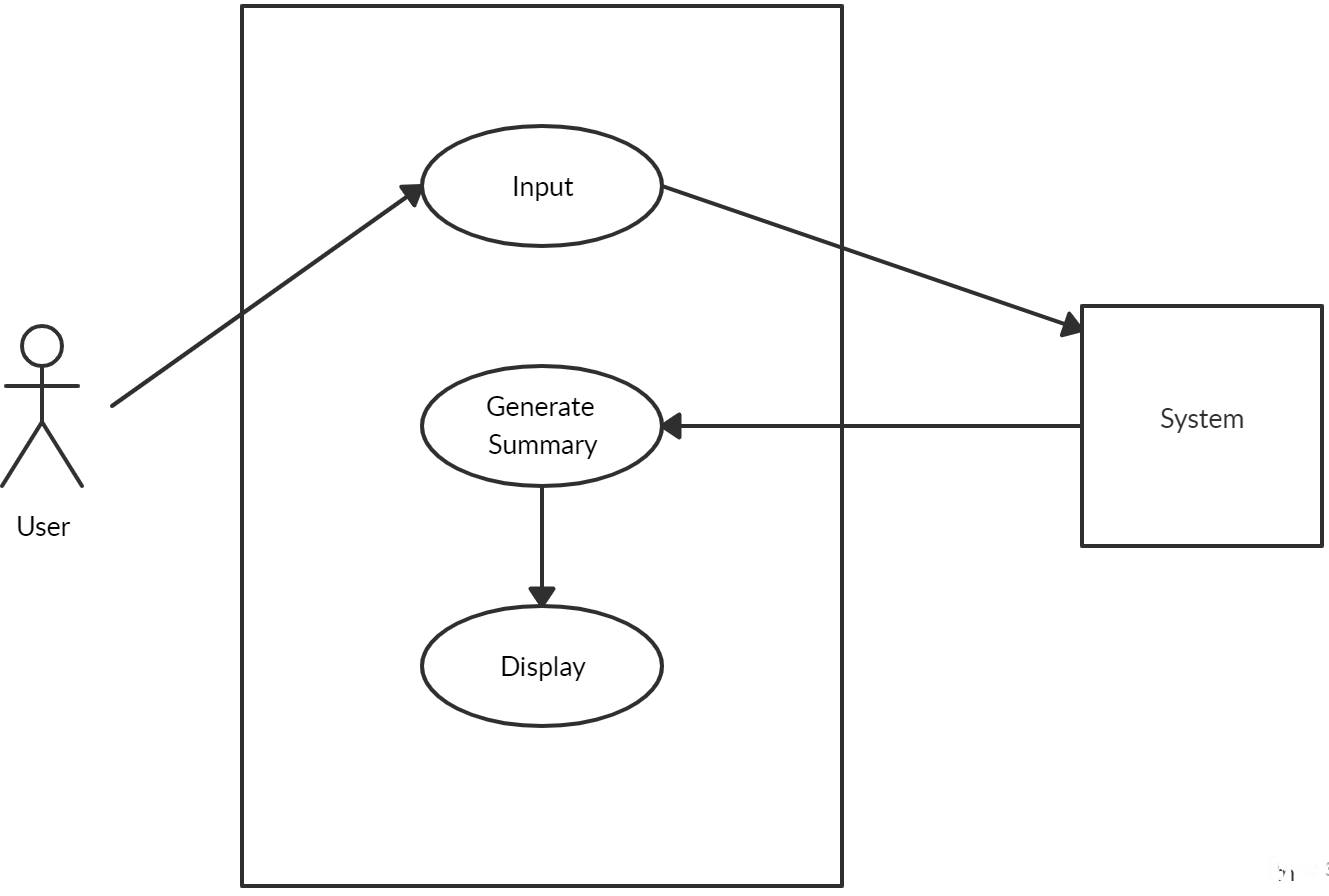
\includegraphics[scale=0.5]{images/SystemOverview.png}
\caption{System Overview}
\label{fig:system overview}
\end{figure}
\pagebreak
\subsection{Product Functions}
The product aims to implement the following functions:
\begin{itemize}
\item Generate an abstractive summary of the available reviews of the selected product using a trained deep learning model.
\item Determine the general sentiment of the users for the selected product.
\item Compute the average rating of the selected product.
\item Display product data including the name, image and price.
\end{itemize}
\subsection{User Classes and Characteristics }
\textbf{End Users}

\begin{itemize}
\item \textbf{Online Shoppers} \\
The application is intended to be used by online shoppers who directly buy goods over the internet. They simply need to have access to the internet and a basic knowledge on using web pages. Increased exposure to technology increases the probability of shopping online and thus using this application.
\item \textbf{Manufacturers} \\
This application can also be used by product manufacturers in order to receive the customers opinions and feedback on their product in brief. They may use this data to improve their strategies and to produce better products which satisfies the customers' needs.
\end{itemize}

\subsection{Operating Environment}
A hardware device like a smartphone, tablet, laptop or desktop with good internet connectivity is required. The user will interact with the system via a web application. The device used to access the system must run on Linux or Windows Operating System.

\subsection{Design and Implementation Constraints}
\begin{itemize}
\item The server must run without a time constraint.
\item Increase in number of reviews affects the computational cost for summarization. 
\item There may be problems with out-of-vocabulary(OOV) words.
\item The language used in the reviews must be English.
\end{itemize}

\subsection{User Documentation}
The system has a simple GUI, so there is no need for additional user documentation. Basic understanding of computers and the internet is sufficient for using this system. 

\subsection{General Constraints}
\begin{itemize}
\item Training of the seq2seq model requires a lot of time depending on the amount of data used.
\item CPU requirements are relatively high and increases with the amount of training data.
\item Training a huge amount of data is infeasible.
\item A stable internet connection is required to use the web application.
\end{itemize}

\subsection{Assumptions and Dependencies}
\begin{itemize}
\item The interface of the system will be easy to use and accessible without any time or location constraints.
\item The user must have an updated web browser.
\item The application assumes a stable network connection.
\item The text parsed by the application is assumed to be in English.
\end{itemize}

\section{External Interface Requirements}
This section describes the user interfaces, hardware interfaces, software interfaces and communication interfaces.

\subsection{User Interfaces}
The user will interact with the system via a web application. The product name will be selected from an auto-complete drop-down list provided in the homepage. 
A ‘Submit’ button will process the input. The output will be displayed as a sweet alert box containing the name, image, price, summary of the reviews, sentiment of the reviews and rating of the product.

\subsection{Hardware Interfaces}
A hardware device like a smartphone, tablet, laptop or desktop with good internet connectivity is required to access the proposed system through a web browser. No specialised hardware is required.

\subsection{Software Interfaces}
The web application is programmed in Python with Flask as the framework for the application. React is used as the front end library along with Javascript. Libraries like Keras and Tensorflow would be used for machine learning and deep learning applications i.e., for training and testing various models. Pandas library would be used to manipulate the data for all computations along with the NLTK library for countless natural language processing of the review text.

\subsection{Communication Interfaces}
The system can be accessed via any popular web browsers like Chrome, Firefox etc. The communication between the application and the web-server will be done using HTTP. The application will send a HTTP request to the web-server. The HTTP POST method will be used to return the response. The web-server returns a HTTP response containing JSON data related to the request.

% \newpage
\section{Hardware and Software Requirements}
This section includes the hardware and software requirements of the proposed system.

\subsection{Hardware Requirements}

\begin{itemize}
\item System: \textbf{CPU - 2.4GHz} (Minimum)
\\Model training and generating abstractive summary consumes a lot of system resources. Therefore a server with Clock speed of at least 2.4GHz is required. \\

\item RAM: \textbf{10GB} (Minimum) \\
The system deals with a large amount of memory requirements in order to train the model. Hence a RAM of at least 10GB is required. \\

\item Hard Disk: \textbf{50GB} (or higher) \\
The system deals with a large amount of data. Hence it requires a hard disk of 50GB.
\end{itemize} 

\subsection{Software Requirements}

\begin{itemize}
\item Operating System: Any operating system (preferably Linux (64-bit), Windows) \\
Linux, Windows is preferred because these are developer friendly, has a powerful shell, flexible and is the most popular  \\

\item Language: \textbf{Python 3.6.2, JavaScript}
\begin{itemize}
    \item \textbf{Python} \\
    Python is an interpreted, high-level, general-purpose programming language. It takes very less time to develop. It is typically 3-5 times shorter than other equivalent programming languages. It has powerful polymorphic list and dictionary types, for which rich syntactic support is built straight into the language.
    \item \textbf{JavaScript} \\
    JavaScript, often abbreviated as JS, is a  high-level programming language, often just-in-time compiled, and multi-paradigm. It has curly-bracket syntax, dynamic typing, prototype-based object-orientation, and first-class functions. JavaScript is the programming language of HTML and the Web.
\end{itemize}

\newpage
\item Frameworks: \textbf{Flask}
\begin{itemize}
    \item \textbf{Flask} \\
    Flask is a python framework used for building the Web interface. Flask is much more fully featured than other frameworks. Python Flask framework supports the use of human-readable website URLs. It also has its own bootstrapping tool. Flask separates a project into individual applications, where Pyramid and Django expect a project to be a single “application” with several views or models.
\end{itemize}

\item IDE: \textbf{Google Colaboratory, Visual Studio Code}
\begin{itemize}
    \item \textbf{Google Colaboratory} \\
    Google Colaboratory is a free cloud service by Google and supports free GPU. It provides us with a cloud environment consisting of n1-highmem-2 instance machine type, 2 virtual CPU at 2.2GHz, 13GB RAM and  64GB Free Space. It has an idle cut-off 90 minutes and can be used to run code for free maximum for 12 hours. 
    \item \textbf{Visual Studio Code} \\
    Visual Studio Code is a source-code editor developed by Microsoft for Windows, Linux and macOS. It includes support for debugging, embedded Git control, syntax highlighting, intelligent code completion, snippets, and code refactoring. 
\end{itemize}

\item Libraries:
\begin{itemize}
    \item \textbf{pandas}
    \item \textbf{Keras}
    \item \textbf{TensorFlow}
    \item \textbf{sklearn}
    \item \textbf{NLTK}
    \item \textbf{pickle}
    \item \textbf{React}
    \item \textbf{json}
    \item \textbf{numpy}
    \item \textbf{BeautifulSoup}
    \item \textbf{sweetalert}
\end{itemize}
\end{itemize}

\newpage
\section{Functional Requirements}
This section briefly describes the functional requirements of the system.

\subsection{Input Product Name}

\begin{figure}[h]
\centering
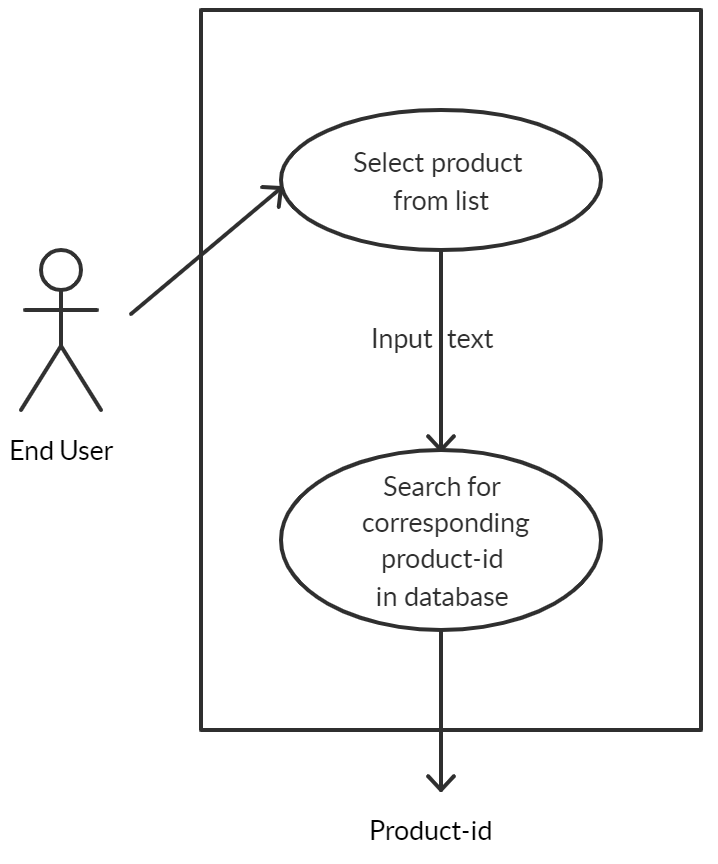
\includegraphics[scale=0.5]{images/input_usecase.png}
\caption{Usecase Diagram - Input Product Name}
\label{fig:usecase1}
\end{figure}

\begin{itemize}
\item The user inputs the product name via the auto-complete drop-down list provided in the web application.
\item The input product name is mapped to its product ID. 
\item The product ID is then retrieved as partial output of this stage. 
\end{itemize}

\subsection{Search for Reviews}

\begin{figure}[H]
\centering
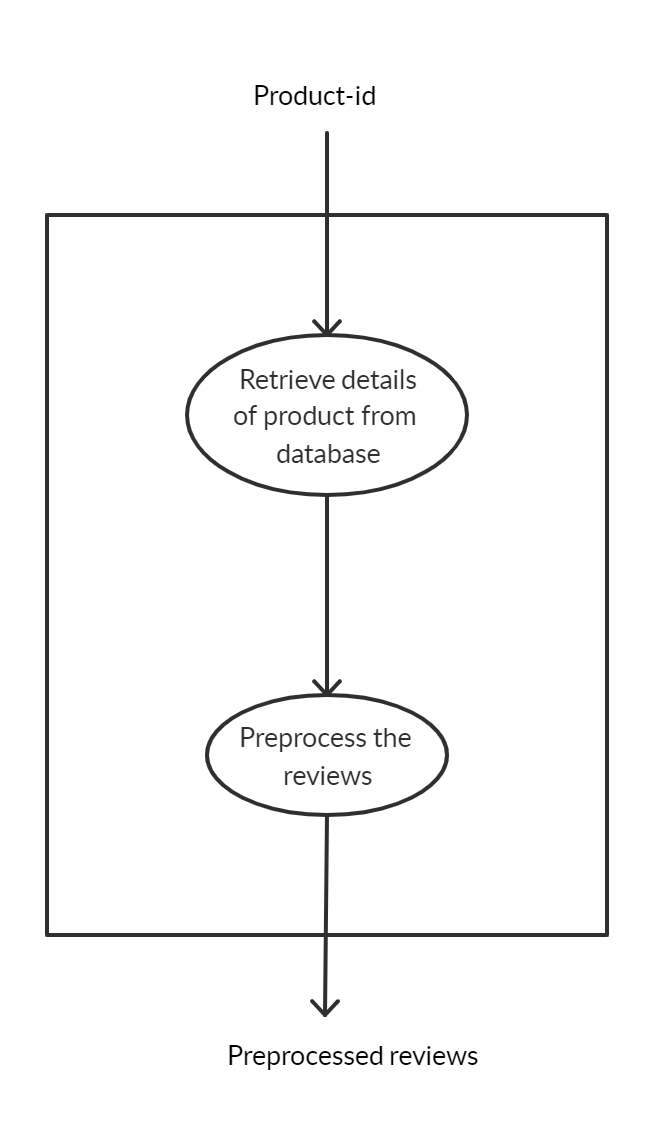
\includegraphics[scale=0.5]{images/search_usecase.png}
\caption{Usecase Diagram - Search Reviews}
\label{fig:usecase2}
\end{figure}

\begin{itemize}
\item The product ID is given as input to this stage.
\item The product database is searched using this product ID to retrieve relevant reviews of the product. 
\item The review data from the database is then given for preprocessing.
\end{itemize}

\subsection{Preprocessing}

\begin{figure}[H]
\centering
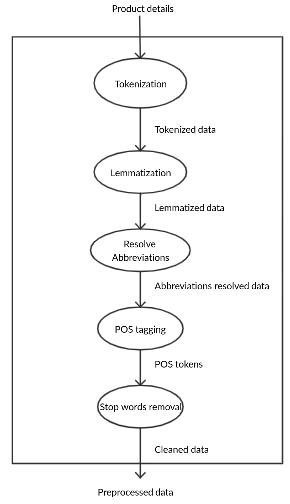
\includegraphics[scale=0.85]{images/preprocessing_usecase.png}
\caption{Usecase Diagram - Preprocessing}
\label{fig:usecase3}
\end{figure}

\begin{itemize}
\item The collected review data is given as input to this stage.
\item The data undergoes tokenization, lemmatization, resolution of abbreviations, POS tagging and removal of stop words.
\item Preprocessed data is obtained as output for this stage.
\end{itemize}

\subsection{Sentiment Analysis}
\begin{figure}[H]
\centering
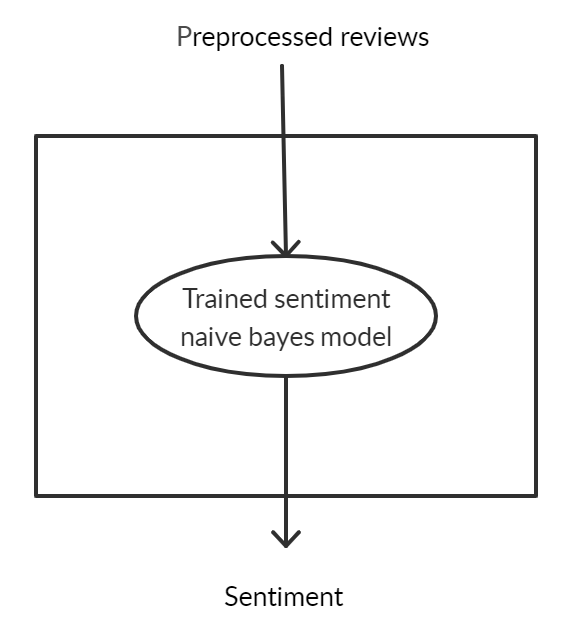
\includegraphics[scale=0.5]{images/sentiment_usecase.png}
\caption{Usecase Diagram - Sentiment Analysis}
\label{fig:usecase4}
\end{figure}

\begin{itemize}
    \item The preprocessed data is fed into the trained Naive Bayes machine learning model for sentiment analysis.
    \item The sentiment of the preprocessed data is generated, which is given to the web application.\\ 
\end{itemize}

\pagebreak

\subsection{Summary Generation}
\begin{figure}[h]
\centering
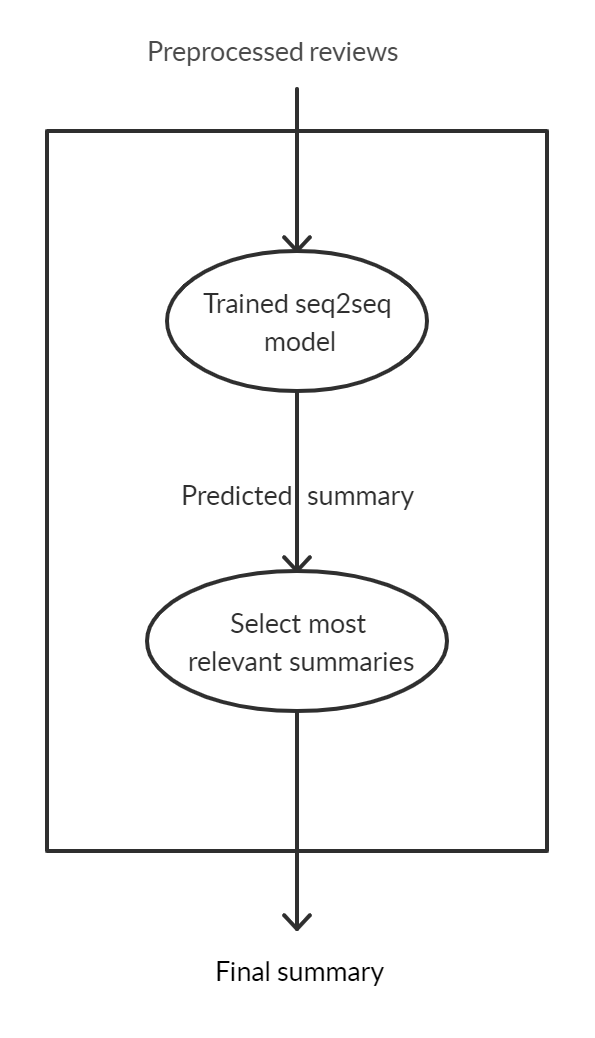
\includegraphics[scale=0.5]{images/summary_usecase.png}
\caption{Usecase Diagram - Summary Generation}
\label{fig:usecase5}
\end{figure}

\begin{itemize}
\item Preprocessed data is fed into the trained machine learning model for generating summary.
\item A summary is generated by the model, which is then given to the web application.
\end{itemize}


\subsection{Display Output}

\vspace{0.5cm}
\begin{figure}[H]
\centering
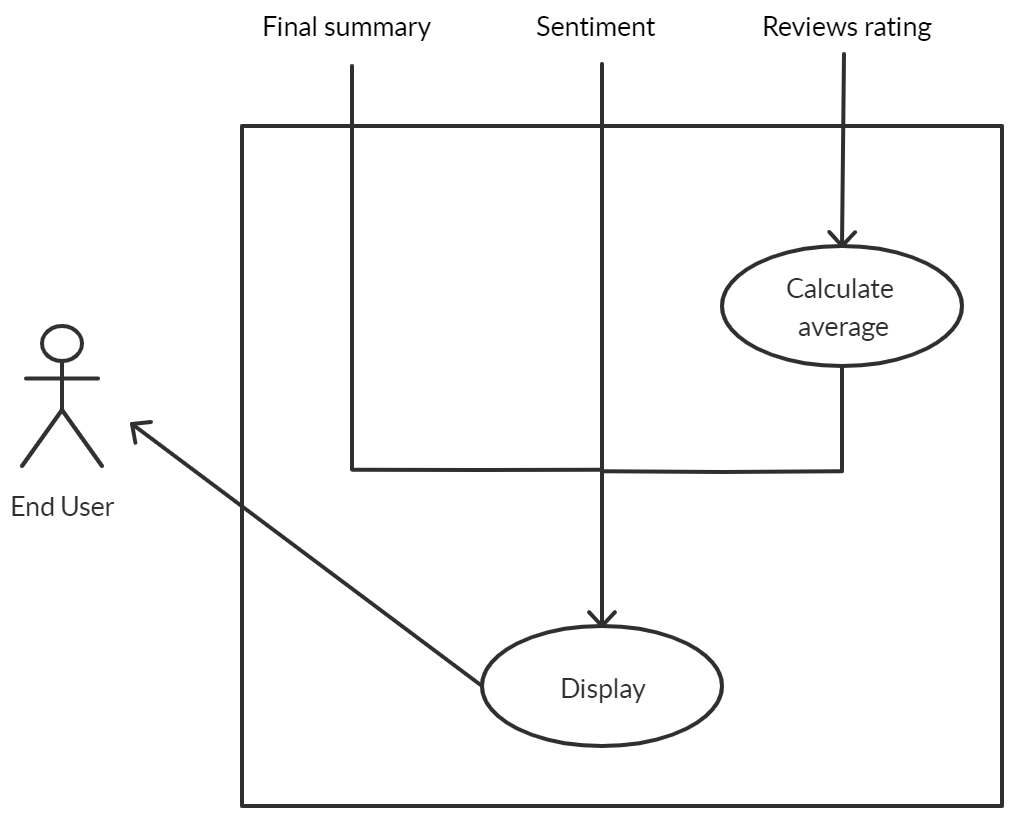
\includegraphics[scale=0.5]{images/output_usecase.png}
\caption{Usecase Diagram - Display Output}
\label{fig:usecase6}
\end{figure}

\begin{itemize}
    \item The summary and the sentiment found from the trained model along with the basic information of the product is sent back to the web application.
    \item The details are displayed in the user interface components. 
\end{itemize}

\newpage
\section{Non-Functional Requirements}    
This section describes performance requirements, safety requirements, security requirements and software quality attributes.

\subsection{Performance Requirements}
The time required to generate the output of the search should be minimum. The literal quality of the summary generated must be high. The summary generated must consider all aspects of the reviews, providing required weightages to important parts. 

\subsection{Security Requirements}
The data given by the user is passed onto a secure server. HTTPS is used to establish the communication protocol. Data mining should not cause security breaches. So, precautions must be taken beforehand in terms of access and permissions. 

\subsection{Software Quality Attributes}
\begin{itemize}

\item \textbf{Reliability}: The website can be used by multiple users concurrently. Any user can access the website.
\item \textbf{Availability}: The system will be available 24 hours a day.
\item \textbf{Maintainability}: The system is implemented as modules thus enhancing its maintainability.
\item \textbf{Portability}: User can use the website at any time, anywhere as long as there is a stable internet connection.
\end{itemize}

\section{Other Requirements} 
Besides the functional and non-functional requirements, there are also other requirements like ease of use and error tolerance. Ease of use describes the ease with which users can interact with the system and error tolerance says about the extent to which error is tolerated if it occurs in the system.

\subsection{Ease of Use}
\begin{itemize}
\item The system will be easy to handle with minimum delay.
\item The system provides an easy and friendly web user interface.
\end{itemize}

\subsection{Error Tolerance}
\begin{itemize}
\item The system should have minimum accuracy level maintained in summary generation.
\item It should be free from processing delays.
\end{itemize}

\chapter{System Design}
\section{System Architecture} 
The system is divided into 6 phases: \\
\begin{itemize}
    \item \textbf{Phase 1} - Training the machine learning models \\
    \item \textbf{Phase 2} - Input data \\
    \item \textbf{Phase 3} - Data collection \\
    \item \textbf{Phase 4} - Data preprocessing \\
    \item \textbf{Phase 5} - Summary generation and sentiment analysis \\
    \item \textbf{Phase 6} - Output display \\
\end{itemize}

\begin{figure}[H]
\centering
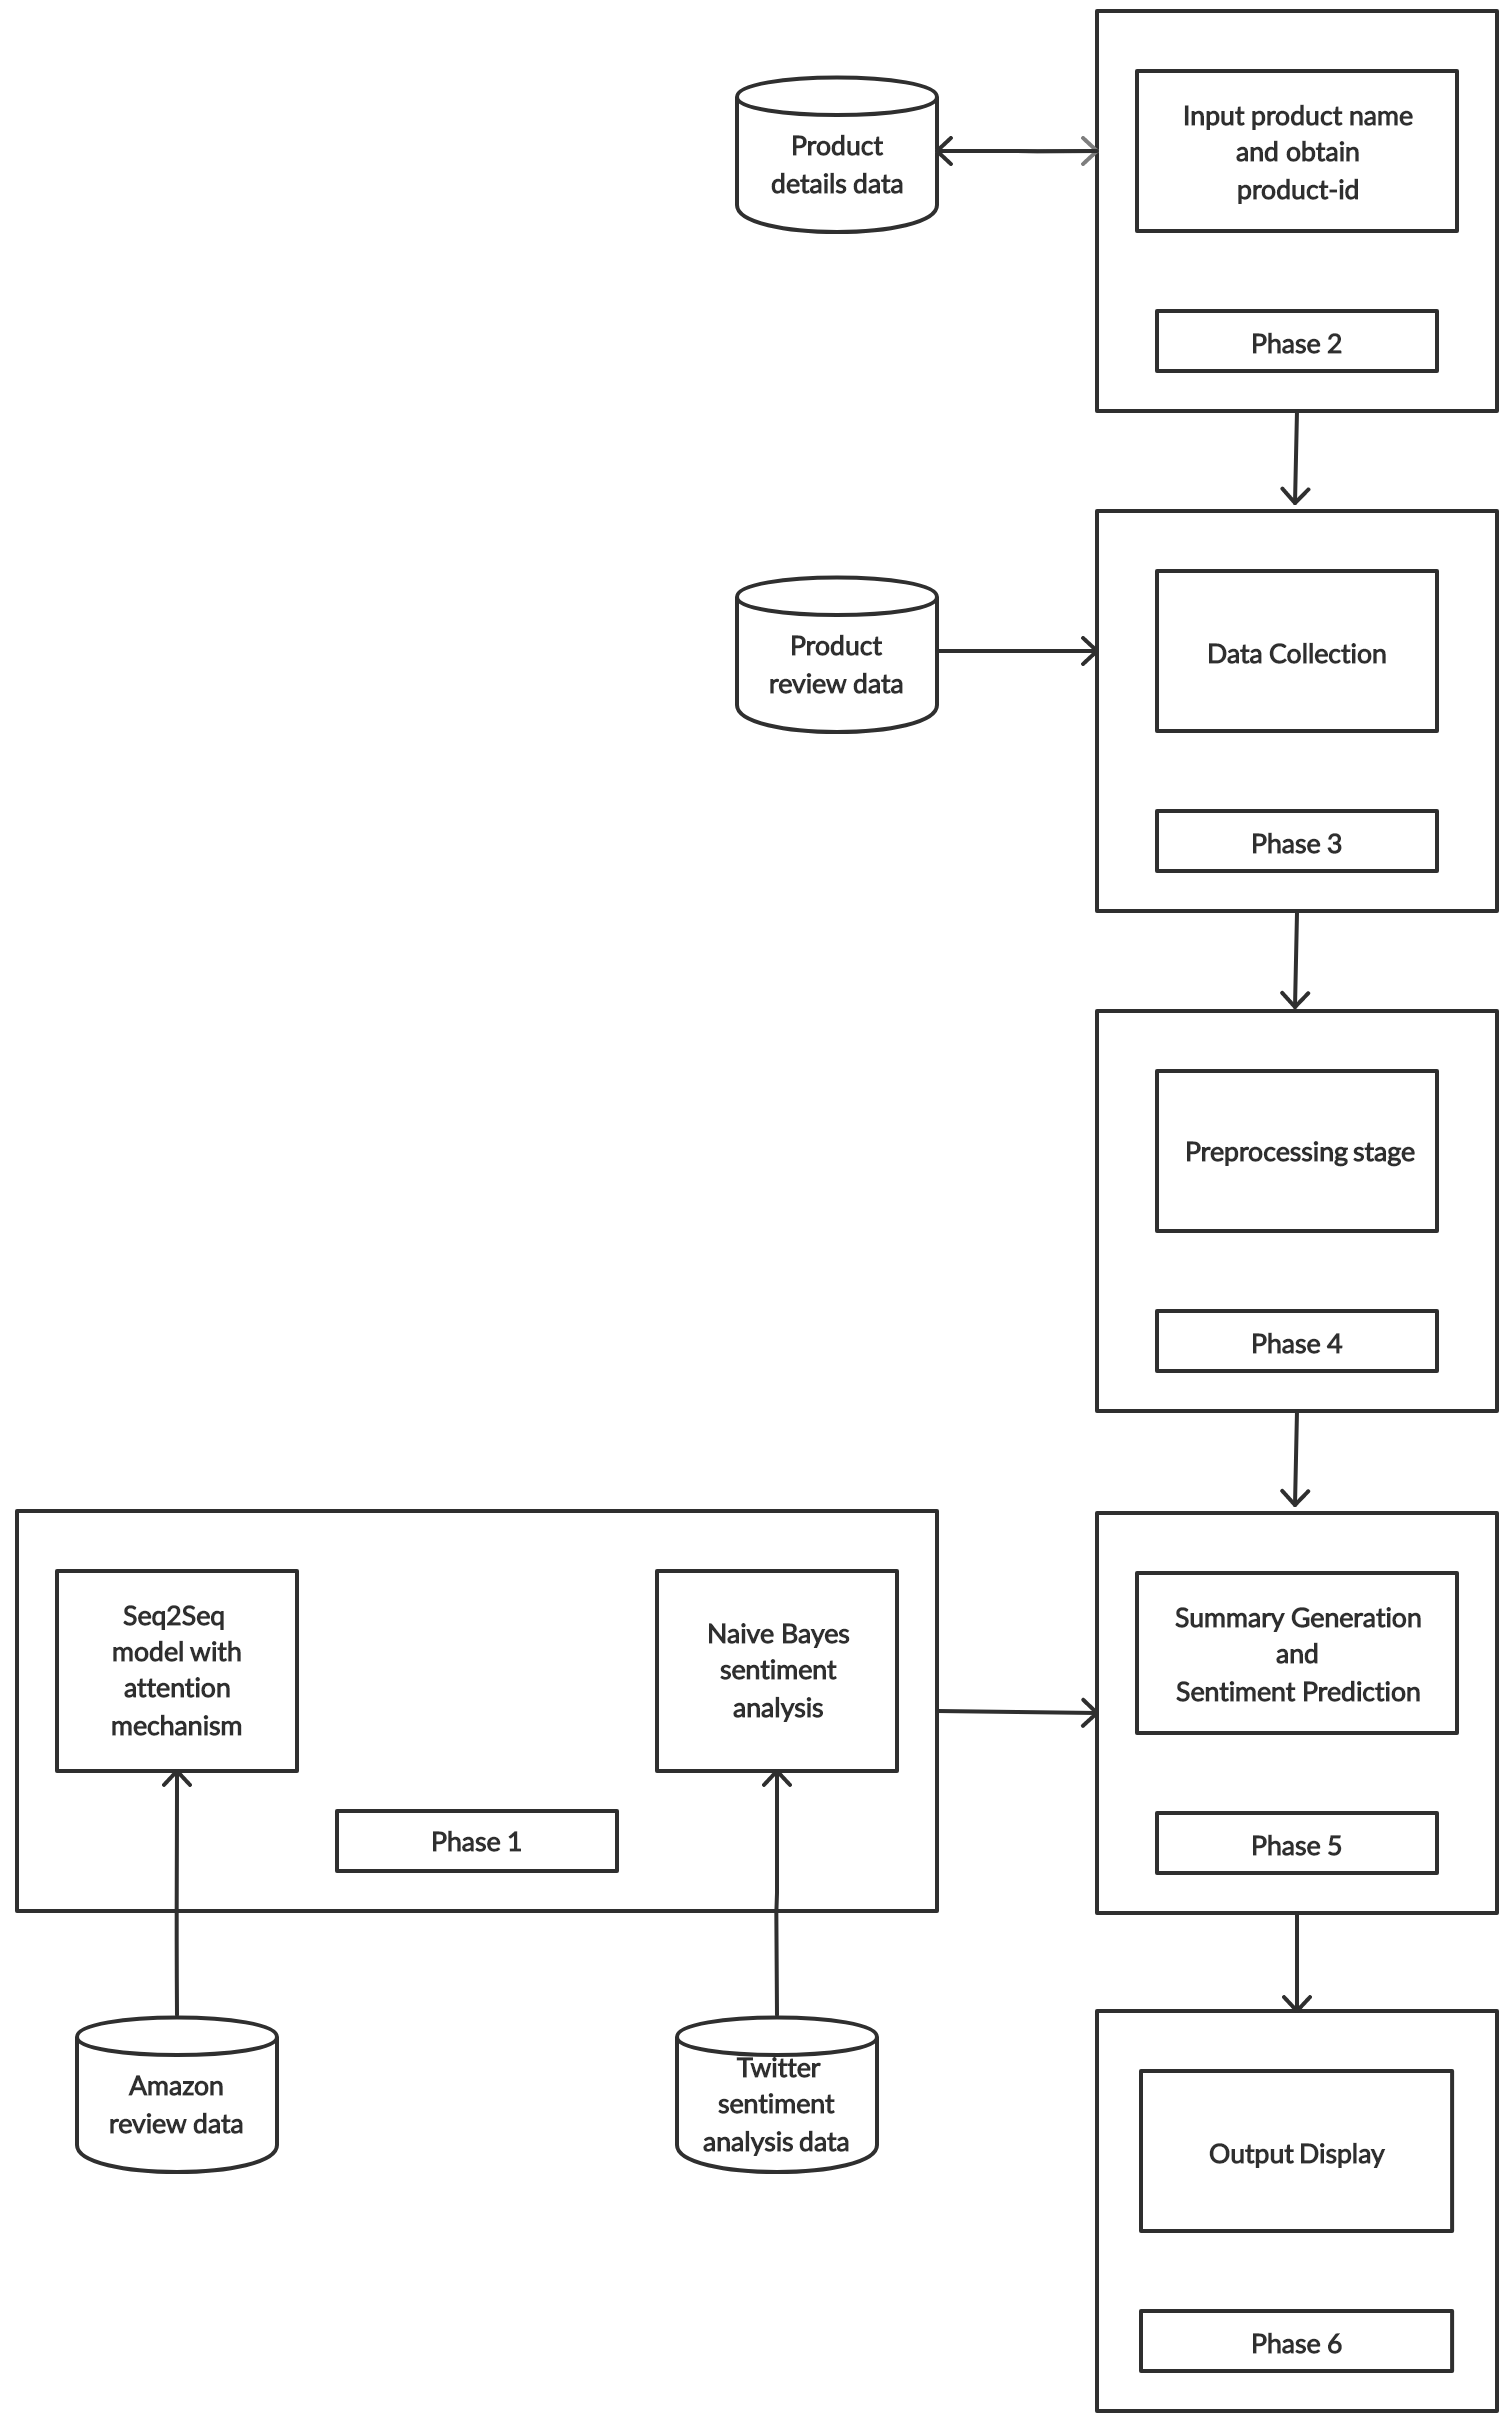
\includegraphics[scale=0.33]{images/system_architecture.png}
\caption{System Architecture}
\label{fig:sysarch}
\end{figure}



\subsection{Training the Models}
There are 2 machine learning models used in the system. One, to produce the summary of reviews and the other, to identify the sentiment of the reviews. A data set containing nearly 6,00,000 reviews of Amazon products and their summaries are fed into a Seq2Seq model with attention mechanism that includes an encoder, a decoder and an attention layer. The data set is used to train the model to produce summary of each review. This trained model is tested with a testing dataset of reviews to check its performance. The model is then stored for use to summarize the required reviews.\\

The Twitter sentiment analysis dataset, which contains tweets and their associated sentiment is used to train a Naive Bayes model to correctly identify the sentiment of any given sentence. The model is tested with sample sentences to check its accuracy. \\

\subsection{Input Data}
In an information system, the input is raw data that is processed to produce the output. The end user inputs the name of the product whose review summary is to be generated. The input is given via an auto-complete drop-down. The name of the product is mapped to its product ID and the same is sent to the next module. 

\subsection{Data Collection}
Data is extracted from the product database using the product ID. The reviews about the selected product is collected and sent into the next phase which is the preprocessing stage. 

\subsection{Data Preprocessing}
Preprocessing is done to obtain a more digestible form so that the machine learning algorithms can perform better. This phase includes tokenization, stop words elimination, lemmatization, POS tagging and resolution of abbreviations. This cleans up the data and converts it into an integer sequence which the model understands. 

\subsection{Summary Generation and Sentiment Analysis}
Preprocessed data is fed into the trained seq2seq model for summary generation. A summary is generated by the model, which is then given to the web application. The summary generated is an abstractive summary, which generates new phrases and sentences that represent the most important information from the source text. The most relevant summaries are selected to be sent to the web application. \\

Preprocessed data is also sent to the sentiment analysis model. The percentage of positive and negative sentiment acquired from all the preprocessed reviews is generated and sent to the web application. 

\subsection{Output Display}
The generated summary and the sentiment is sent to the web application. The details are presented to the user through a sweet alert. It contains the name, image, price, summary, rating and sentiment of the selected product. 


\section{Data Description}
\subsection{Database Design}
\begin{figure}[H]
\centering
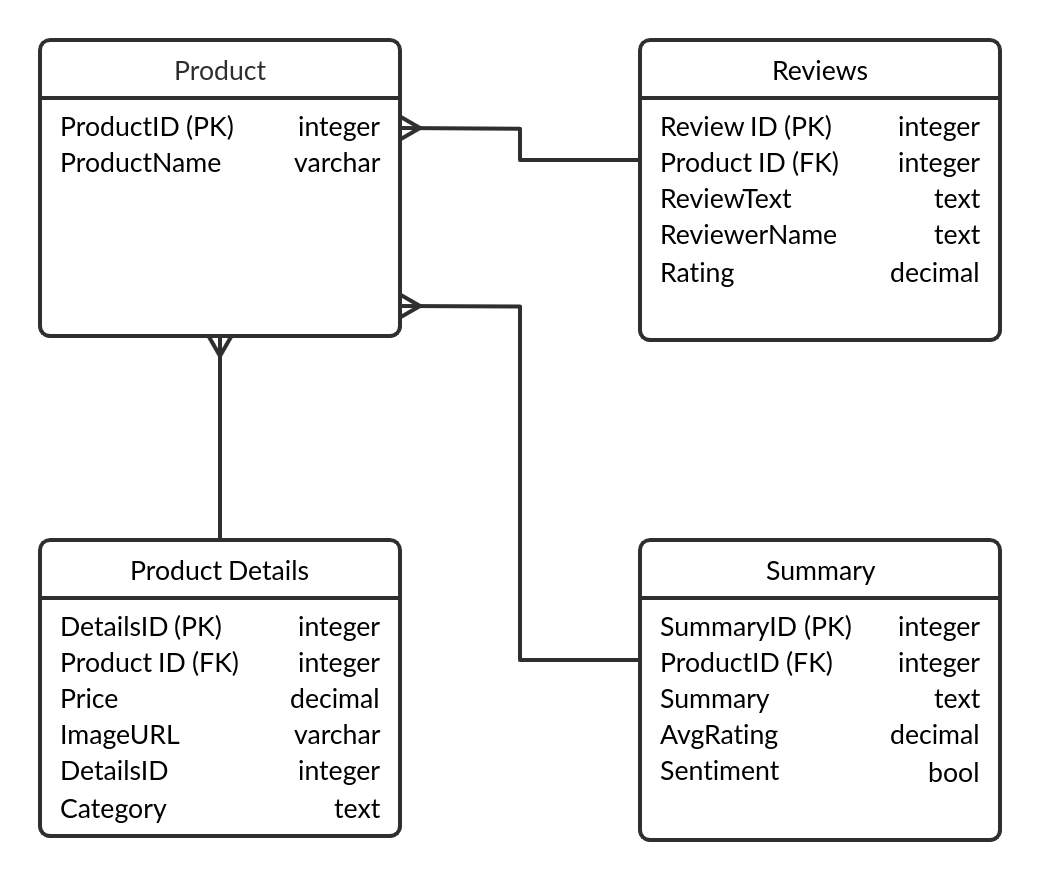
\includegraphics[scale=0.45]{DatabaseDesign.png}
\caption{Database Design}
\label{fig:fig}
\end{figure}

\newpage

\subsection{Use Case Diagram}

\begin{figure}[hbt!]
\centering
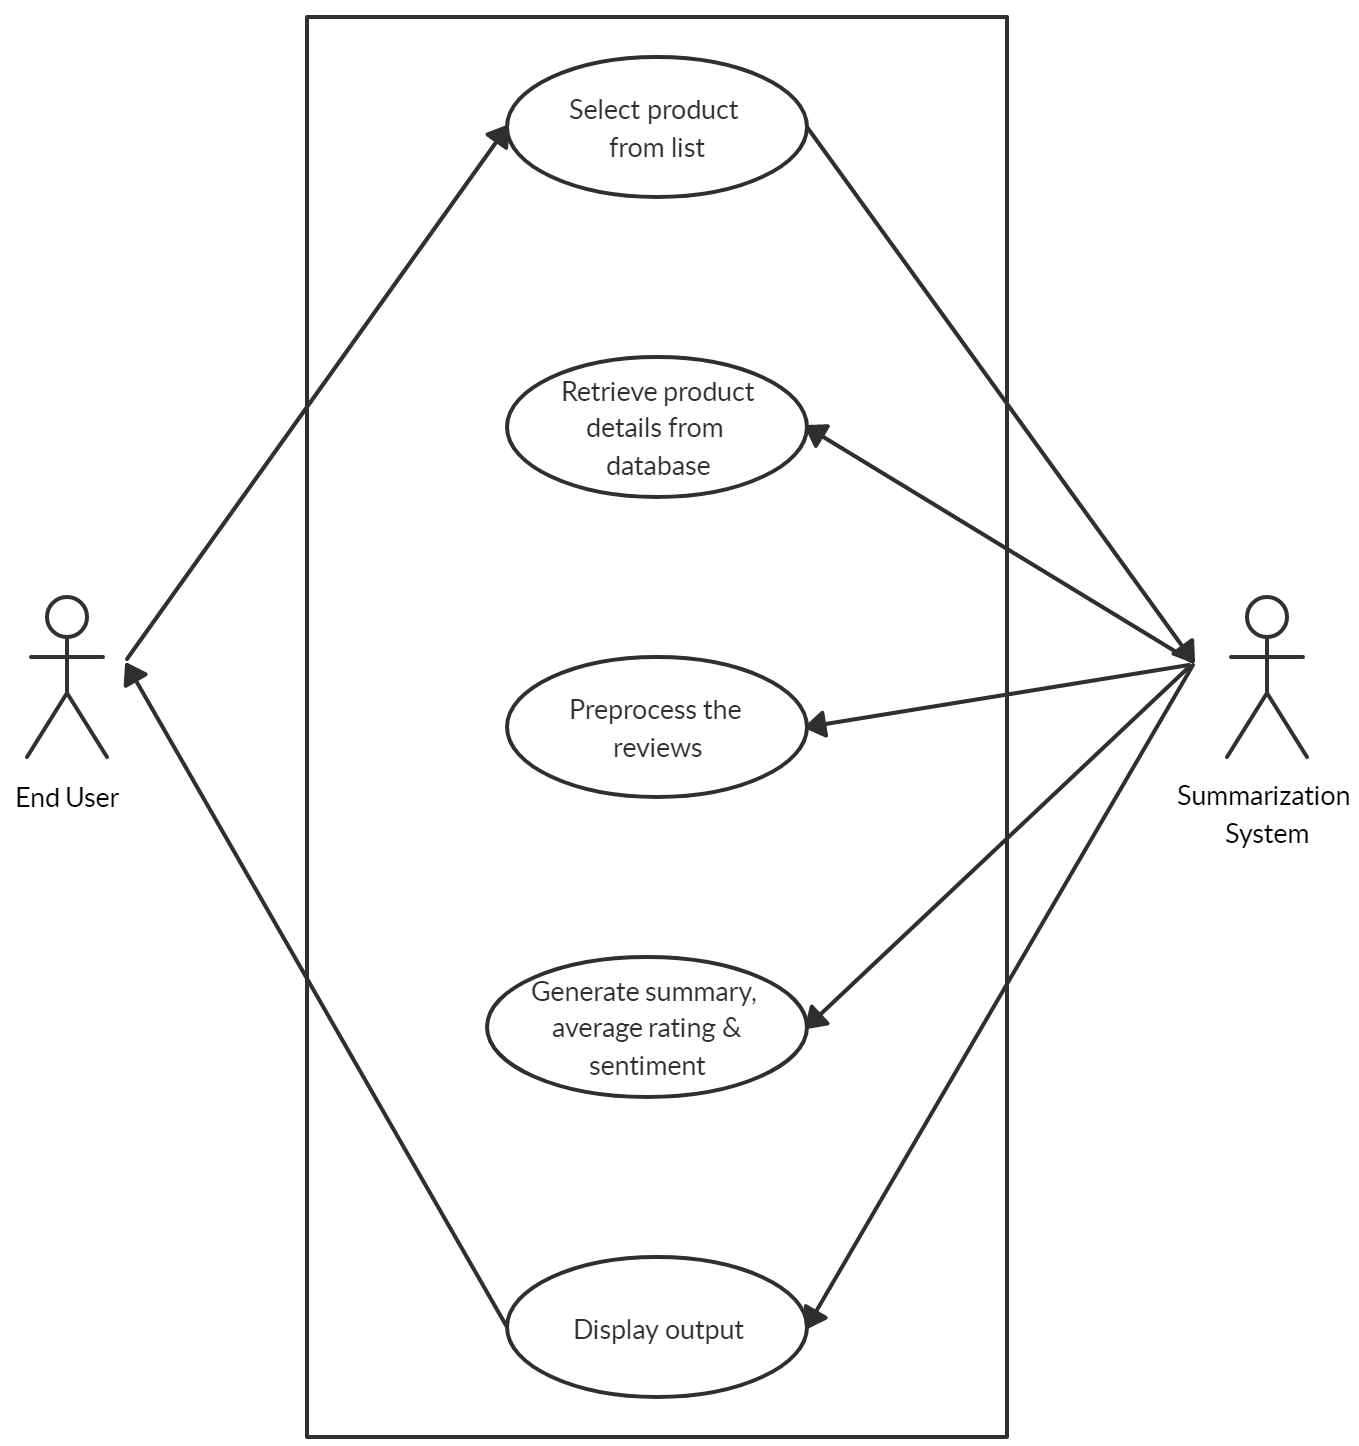
\includegraphics[scale=0.4]{images/usecase.png}
\caption{Usecase Diagram}
\label{fig:usecase1}
\end{figure}

\pagebreak


\clearpage
\subsection{Class Diagram}
\begin{figure}[hbt!]
\centering
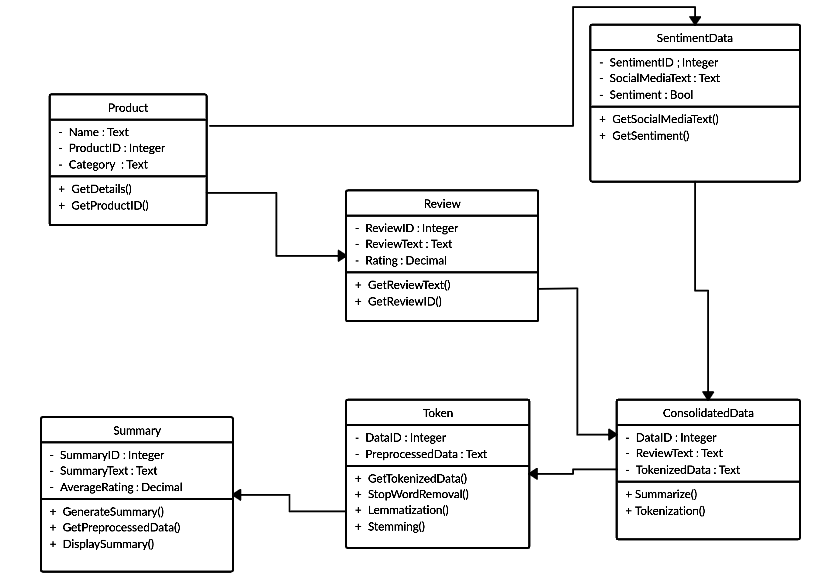
\includegraphics[scale=0.65]{ClassDiagram.png}
\caption{Class Diagram}
\label{fig:classdiagram}
\end{figure}

\clearpage
\subsection{Activity Diagram}
\begin{figure}[hbt!]
\centering
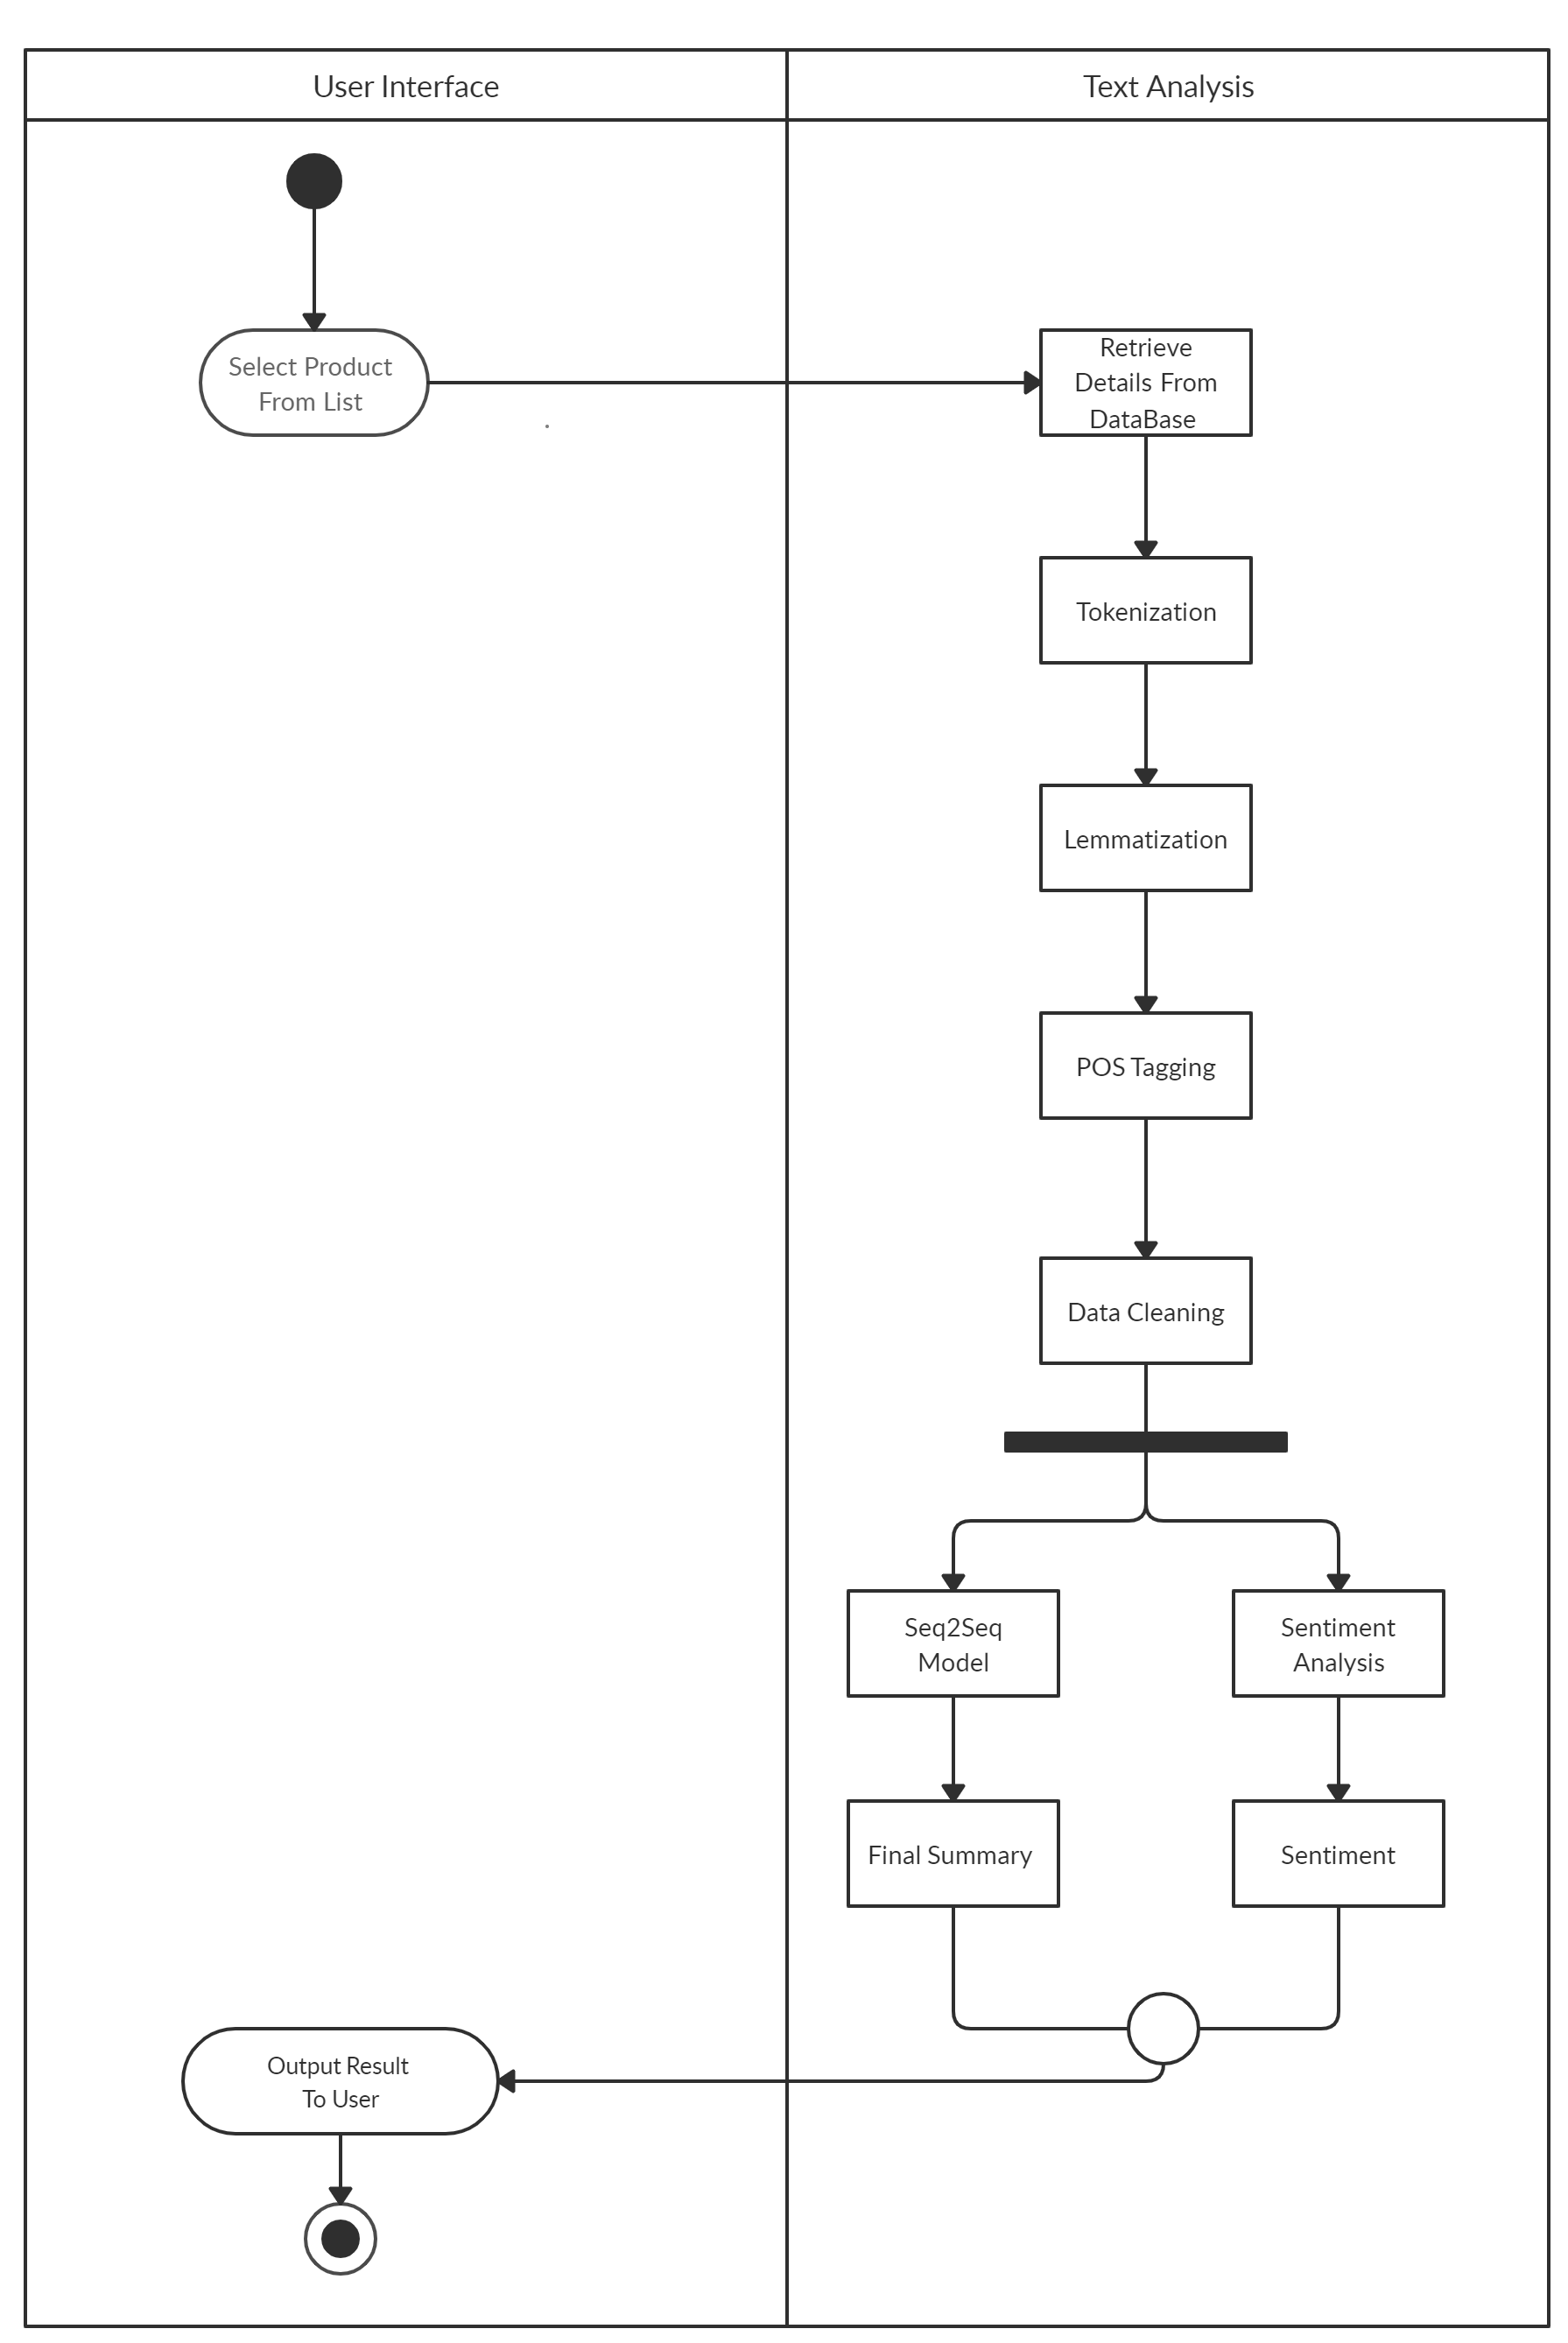
\includegraphics[scale=0.25]{images/ActDiagram.png}
\caption{Activity Diagram}
\label{fig:activitydiagram}
\end{figure}

\pagebreak
\subsection{Dataset Design}
For training the summary generation machine learning model, we to use the Amazon product data\cite{20}, an open source dataset composed of millions of amazon reviews. This dataset contains product reviews and metadata from Amazon, including 142.8 million reviews spanning the period from May 1996 - July 2014. It includes reviews (ratings, text, helpfulness votes), product metadata (descriptions, category information, price, brand, and image features), and links to other relevant data (also viewed/also bought graphs). \\
Twitter is a well-known microblog service that allows public data to be collected via APIs. For training the text sentiment prediction model we make use of the NLTK's twitter corpus currently containing a sample of 20k tweets retrieved from the Twitter Streaming API. 


\section{Libraries and Packages Used}

\subsection{pandas}
In computer programming, pandas is a software library written for the Python programming language for data manipulation and analysis. In particular, it offers data structures and operations for manipulating numerical tables and time series. It has intelligent data alignment and integrated handling of missing data.

\subsection{Keras}
Keras is an open-source neural-network library written in Python. It is capable of running on top of TensorFlow, Microsoft Cognitive Toolkit, R, Theano, or PlaidML. Designed to enable fast experimentation with deep neural networks, it focuses on being user-friendly, modular, and extensible. Keras has strong multi-GPU \& distributed training support.

\subsection{TensorFlow}
TensorFlow is a free and open-source artificial intelligence software library for dataflow and differentiable programming across a range of tasks. It is a symbolic math library, used for machine learning applications such as to create large-scale neural networks with many layers. It uses data flow graphs to build models. TensorFlow is helpful for Classification, Perception, Understanding, Discovering, Prediction and Creation.

\subsection{sklearn} 
Scikit-learn is a free machine learning library for Python. It features various algorithms like support vector machine, random forests, and k-neighbours. It also supports Python numerical and scientific libraries like NumPy and SciPy. The sklearn library contains a lot of efficient tools for machine learning and statistical modeling including classification, regression, clustering and dimensionality reduction.

\subsection{NLTK}
NLTK (Natural Language ToolKit) provides a suite of text processing libraries for classification, tokenization, stemming, tagging, parsing, and semantic reasoning like nltk.sent-tokenization, nltk.word-tokenization, nltk.stopwords etc. When compared to other libraries like spacy, genism, scikit-learn, NLTK has many advantages such as fast tokenization, plenty of approaches to each nlp task, and it supports a large number of languages.

\subsection{React}
React is an open-source Javascript library that is used to build user interfaces. It helps build encapsulated components that manage their own state, then compose them to make complex UIs. React abstracts away the DOM from you, offering a simpler programming model and better performance. 

\subsection{json}
Python has a built-in package called json, which can be used to work with JSON data. json exposes an API familiar to users of the standard library marshal and pickle modules. The package contains all the functions that will help one use the JSON files and the allied activities.

\subsection{pickle}
Python pickle module is used for serializing and deserializing a Python object structure. Any object in Python can be pickled so that it can be saved on disk. What pickle does is that it “serializes” the object first before writing it to file. Pickling is a way to convert a python object (list, dict, etc.). The module is used to save trained models in storable formats.

\subsection{numpy}
NumPy is a library for the Python programming language, adding support for large, multi-dimensional arrays and matrices, along with a large collection of high-level mathematical functions to operate on these arrays.

\subsection{BeautifulSoup}
Beautiful Soup is a Python package for parsing HTML and XML documents. It creates a parse tree for parsed pages that can be used to extract data from HTML, which is useful for web scraping. It is available for Python 2.7 and Python 3.

\subsection{sweetalert}
SweetAlert is a package in npm used to create beautiful, responsive and customized alerts in web applications. It gives you different options according to the need.

\pagebreak
\section{Module Description}

\subsection{Data Collection}
\begin{itemize}
    \item Amazon product dataset is downloaded for the Seq2Seq summarization model.
    \item Dataset of positive and negative tweets available in the NLTK library is downloaded for training sentiment analysis model.
\end{itemize}

\subsection{Preprocessing}
\begin{itemize}
    \item The dataset is divided into training set and test set.
    \item Reviews from the training set and test set are preprocessed.
    \item Tokenization of sentences and words is done with the functions in NLTK library.
    \item Stop words are removed using the NLTK corpus of stop words.
    \item Unnecessary punctuation marks are eliminated.
    \item Abbreviations are resolved by replacing them with their full forms.
    \item Lemmatization is carried out to obtain the root word with respect to the context.
    \item The preprocessed training data is then used for training the model and the preprocessed testing data is used for testing the model.
\end{itemize}

\subsection{Training and Testing the Models}
\begin{itemize}
    \item The Seq2Seq model with Attention Mechanism is developed by defining its encoder-decoder architecture and the attention layer.
    \item The model is trained with the preprocessed review data
    \item The model is tested using the preprocessed testing review data.
    \item The model is then saved in .h5 format.
    \item The Naive Bayes model is trained with the preprocessed Twitter sentiment data.
    \item Preprocessed testing review data is then fed into the model to obtain the sentiments.
    \item This model is also saved and stored as a pickle file.
\end{itemize}

\subsection{Input Module}
\begin{itemize}
\item User Interface is built using React.
\item The input is received through an auto-complete drop-down list.
\item The product name is mapped to the product ID and is sent to the back-end of the application.
\end{itemize}

\subsection{Summary Generation and Sentiment Analysis}
\begin{itemize}
\item The product ID is used to retrieve the reviews from the product dataset.
\item The reviews are preprocessed and fed into the summarization model to produce summary of each review.
\item The preprocessed reviews are fed into sentiment analysis model to obtain the sentiment.
\item The most relevant review summaries are returned to the web application along with the sentiment factor.
\end{itemize}

\subsection{Output Display}
\begin{itemize}
\item The summary and sentiment along with the basic details of the product is displayed.
\item A sweet alert box is used for the same.
\end{itemize}

\chapter{Data Flow Diagram}
\section{Level 0 DFD}
\begin{figure}[hbt!]
\centering
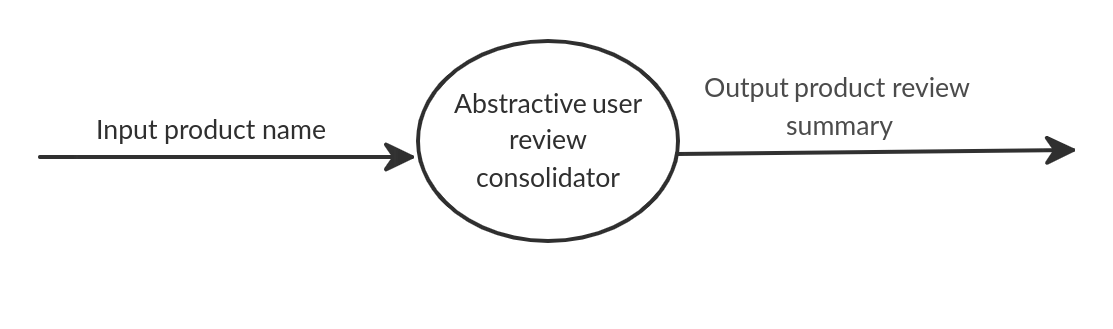
\includegraphics[scale=0.4]{DFDlevel0.png}
\caption{DFD Level 0}
\label{fig:dfd0}
\end{figure}

\section{Level 1 DFD}
\begin{figure}[hbt!]
\centering
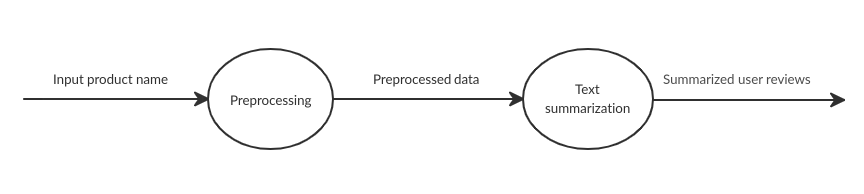
\includegraphics[scale=0.6]{DFDlevel1.png}
\caption{DFD Level 1}
\label{fig:dfd1}
\end{figure}

\newpage
\section{Level 2 DFD}
\begin{figure}[hbt!]
\centering
\includegraphics[scale=0.3]{images/DFDLevel2.png}
\caption{DFD Level 2}
\label{fig:dfd2}
\end{figure}

\chapter{Implementation}
\section{Algorithms}
\subsection{Algorithm for Inputting Product Name}
\vspace{0.5cm}
\begin{algorithm}[H]
\SetAlgoLined
\KwIn{Product name}
\KwOut{Product ID }
Start \\
Accept product name from the drop-down list\\
\eIf{user selected x}{
   Retrieve the product ID from the database\\
   Send the product ID to the back-end server\\
   }
   {
   Prompt the user to try again\\
   Go to step 2\\
   }
Stop \\
\caption{Algorithm for Inputting Product Name}
\end{algorithm}
\vspace{0.5cm}

\subsection{Algorithm for Data Collection}
\vspace{0.5cm}
\begin{algorithm}[H]
\SetAlgoLined
\KwIn{The product ID}
\KwOut{Reviews corresponding to the product ID}
Start \\
Initialise pid with product id of the chosen product \\
Initialise df as product details dataset\\
Initialise result as an empty dataframe \\
\For{every row in df}{
    \If{product-id at the selected row is same as pid}{
    Append the row to result\
    }
}
Return result \\
Stop \\
\caption{Algorithm for Data Collection}
\end{algorithm}
\vspace{0.5cm}

\subsection{Algorithm for Preprocessing}
\vspace{0.5cm}
\begin{algorithm}[H]
\SetAlgoLined
\KwIn{Consolidated review data}
\KwOut{Preprocessed review data}
Start \\
Separate the words in the data into tokens \\
Remove the stop words from the input data \\
Resolve abbreviations in the data \\
Perform lemmatization on the data \\
Stop \\
\caption{Algorithm for Preprocessing}
\end{algorithm}
\vspace{0.5cm}

\subsection{Algorithm for  Training of Seq2Seq Model with Attention Mechanism}
\vspace{0.5cm}
\begin{algorithm}[H]
\SetAlgoLined
\KwIn{Product review dataset, maximum review length, maximum summary length}
\KwOut{Trained abstractive summarization model}
Start \\
Read dataset into a dataframe \\
Preprocess the reviews and summaries from the dataframe \\
Remove rows containing null values from dataframe \\
Remove rows containing reviews or summaries less than the set value \\
Split the training and testing data \\
\textbf{Training phase:} \\
    \Begin 
    {
        Prepare a tokenizer for reviews on training data \\
        Convert review text sequences into integer sequences \\
        Pad the review sequences with zeroes upto max review length \\
        Prepare a tokenizer for summaries on training data \\
        Convert summary text sequences into integer sequences \\
        Pad the summary sequences with zeroes upto max summary length \\
        Append \textless start\textgreater \hspace{0.05cm} and \textless end\textgreater \hspace{0.05cm}  tokens to each sequence \\
        Delete rows with only \textless start\textgreater \hspace{0.05cm}  and \textless end\textgreater \hspace{0.05cm} tokens \\
        Set up the Encoder \\
        Set up the Attention Layer \\
        Set up the Decoder \\
        Train the model till loss values are minimum\\
        Save the model
    }
    \End
\textbf{Inference phase:} \\
    \Begin
    {
        Create dictionary to convert the index to word for target and source vocabulary using the tokenizer \\
        \For{Each review in testing dataset}
        {
            Encode the entire input sequence \\
            Initialize the decoder with the internal states of the encoder \\
            Pass \textless start\textgreater \hspace{0.05cm} token as an input to the decoder \\
            Run the decoder for one time-step with the internal states \\
            Select the word with the maximum probability \\
            Pass the sampled word as an input to the decoder in the next time-step and update the internal states with the current time-step\\
            Repeat steps 30-32 until \textless end\textgreater \hspace{0.05cm} token is generated or maximum length of the target sequence is reached \\
        }
    }
    \End
Stop \\
\caption{Algorithm for Training Seq2Seq Model with Attention Mechanism}
\end{algorithm}
\vspace{0.5cm}

\subsection{Algorithm for Naive Bayes Sentiment Analysis Model}
\vspace{0.5cm}
\begin{algorithm}[H]
\SetAlgoLined
\KwIn{Twitter sentiment analysis dataset}
\KwOut{Trained naive bayes model}
Start \\
Read dataset into a dataframe \\
Preprocess the reviews and summaries from the dataframe \\
Remove rows containing null values from dataframe \\
Create an instance of Naive Bayes classifier \\
Train the model with cleaned data \\
Save the model\\
Stop \\
\caption{Algorithm for Naive Bayes Sentiment Analysis Model}
\end{algorithm}
\vspace{0.5cm}


\subsection{Algorithm for Summary Generation}
\vspace{0.5cm}
\begin{algorithm}[H]
\SetAlgoLined
\KwIn{Preprocessed review data}
\KwOut{Product review summary}
Start \\
Initialise df as preprocessed product review data\\
% Initialise n as number of rows in df \\
Initialise result as empty string array \\
Initialize the decoder with internal states of the encoder \\
Initialise reqlen as length of summary required\\
\For{every row in df}{
    Initialise summary as empty string\\
    \While{$len(result) < reqlength$}{
        % Encode review, df[i].review into vector form\\
        Encode the review into vector form\\
        Run the decoder for one time-step \\
        Calculate the probability for the next word\\
        Select the word with maximum probability \\
        Pass the sampled word as input to the decoder in the next time-step \\
        Update the internal states with the current time-step \\
    }
    Append summary to result\\
}
Let word-frequencies be a dictionary containing frequency of each word in result \\
Score each summary using word-frequencies \\
Select required number of sentences in final summary based on maximum sentence scores\\
Return result\\
Stop \\
\caption{Algorithm for Summary Generation}
\end{algorithm}
\vspace{0.5cm}

\subsection{Algorithm for Sentiment Analysis}
\vspace{0.5cm}
\begin{algorithm}[H]
\SetAlgoLined
\KwIn{Preprocessed review data}
\KwOut{Product review positive and negative sentiment percentages}
Start \\
Initialise df as preprocessed product review data\\
Initialise sent-pos with 0 as value \\
Initialise sent-neg with 0 as value\\
\For{Each row in df}{
    Call trained Naive Bayes Model on review at row i \\
    \eIf{sentiment predicted is positive}{
        sent-pos = sent-pos + 1
        }
        {
        sent-neg = sent-neg + 1
        }
}
Return\[ ( \hspace{0.2cm} \frac{sent-pos \times 100}{n}\ \hspace{0.5cm} and \hspace{0.5cm} \frac{sent-neg \times 100}{n} \hspace{0.2cm} )\]\\
Stop \\
\caption{Algorithm for Sentiment Analysis}
\end{algorithm}
\vspace{0.5cm}


\section{Development Tools}
\begin{itemize}
    \item \textbf{Google Colaboratory} \\
    Google Colaboratory is a free cloud service by Google and supports free GPU. It provides us with a cloud environment consisting of n1-highmem-2 instance machine type, 2 virtual CPU at 2.2GHz, 13GB RAM and  64GB Free Space. It has an idle cut-off 90 minutes and can be used to run code for free maximum for 12 hours.
    \item \textbf{Visual Studio Code} \\
    Visual Studio Code is a source-code editor developed by Microsoft for Windows, Linux and macOS. It includes support for debugging, embedded Git control, syntax highlighting, intelligent code completion, snippets, and code refactoring.
    \item \textbf{Git} \\
    Git is a free and open source distributed version control system designed to handle everything from small to very large projects with speed and efficiency. Compared to other version control systems, Git is responsive, easy to use, and inexpensive (free, actually). Branching allows you to create independent local branches in your code.
    \pagebreak
    \item \textbf{Postman}\\
    Postman is a collaboration platform for API development. Postman's features simplify each step of building an API and streamline collaboration so you can create better APIs faster. It makes it easier for developers to create, share, test and document APIs. This is done by allowing users to create and save simple and complex HTTP/s requests, as well as read their responses.
\end{itemize}

\chapter{Testing}
\section{Testing Methodologies}
Software testing methodologies are the various strategies or approaches used to test an application to ensure it behaves and looks as expected. The idea of using various testing methodologies in the development process is to ensure that the software can successfully work in multiple environments and different platforms. Broadly, this is broken down into functional and non-functional testing. In functional testing, the application is tested against business requirements. Non-functional testing methods incorporate all test types focused on the operational aspects of a piece of software. We have performed functional testing part which includes unit testing, integration testing and system testing, each of which is described below.

\section{Unit Testing}
Unit testing refers to the testing of individual software modules or components that make up an application or system. It validates that each module of the software performs as designed.

\subsection{Input Module}
User selects the required product from the drop-down list.By mapping the product name to its corresponding product id, all reviews for the selected product are extracted.
\begin{figure}[H]
\centering
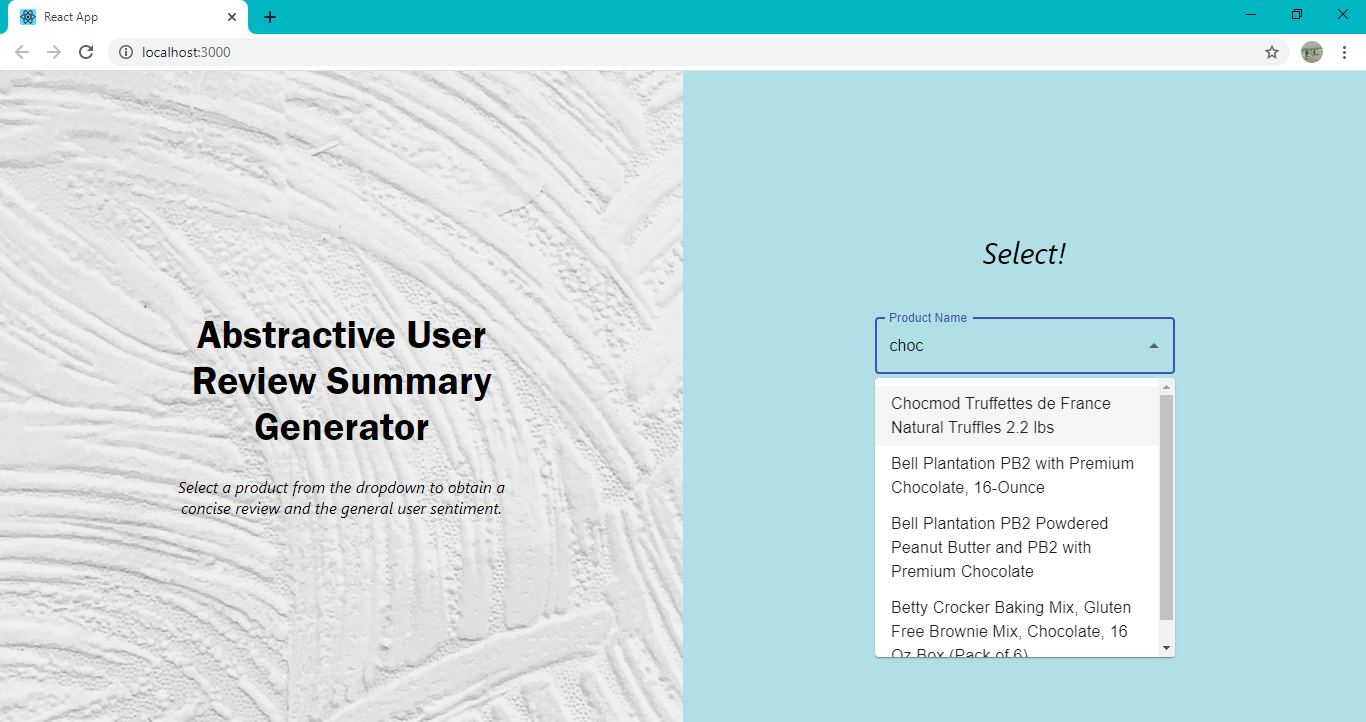
\includegraphics[scale=0.5]{images/dropdown.png}
\caption{Drop-Down Selection}
\label{fig:dropdown}
\end{figure}

\subsection{Preprocessing Module}
The review data undergoes tokenization, removal of stop words, POS tagging and lemmatization. 
\begin{figure}[H]
\centering
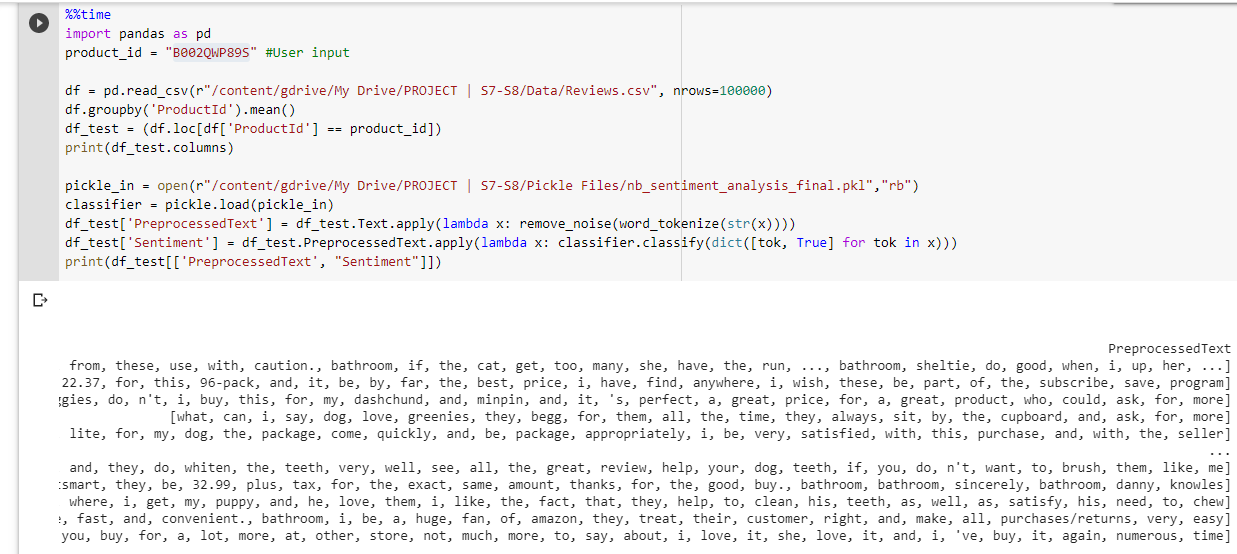
\includegraphics[scale=0.5]{images/Preprocessed Text.png}
\caption{Preprocessed Text}
\label{fig:preprocess}
\end{figure}

\subsection{Model Training}
For the sentiment analysis, the in-built sentiment dataset from nltk is used to train and test a Naive Bayes model.
\begin{figure}[H]
\centering
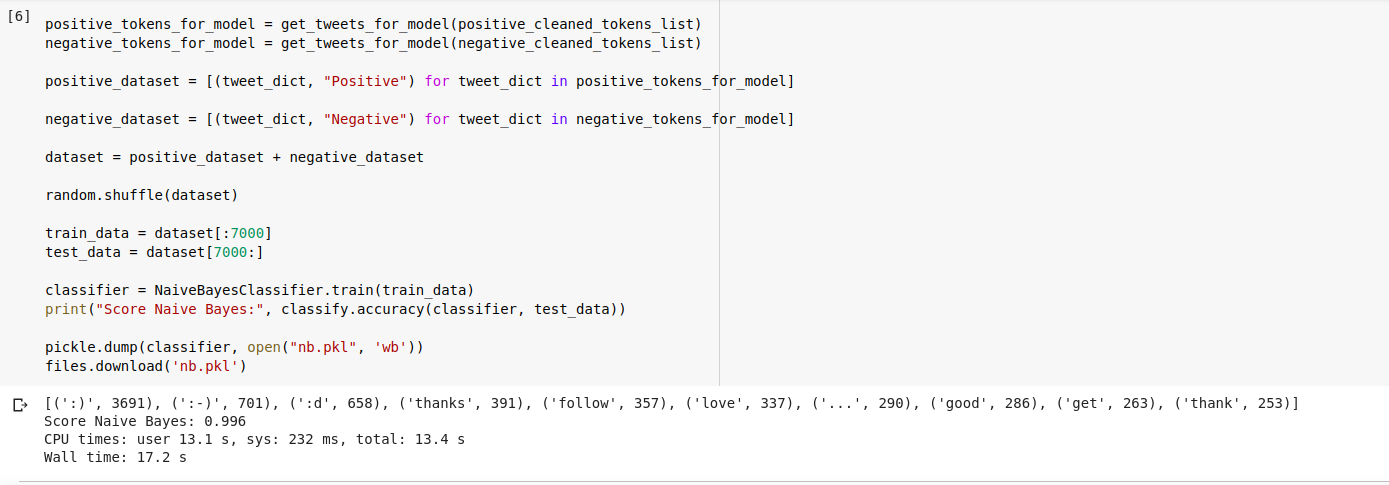
\includegraphics[scale=0.35]{images/sentiment_modeltraining.png}
\caption{Naive Bayes Model for Sentiment Analysis}
\label{fig:sentiment_train}
\end{figure}
Here, we use a Seq2Seq model with attention mechanism that includes an encoder, decoder and attention layer. Amazon product dataset which contains the product reviews and their summaries are fed into the model to train the model to produce summaries. The model is then tested with a testing dataset of reviews.
\begin{figure}[H]
\centering
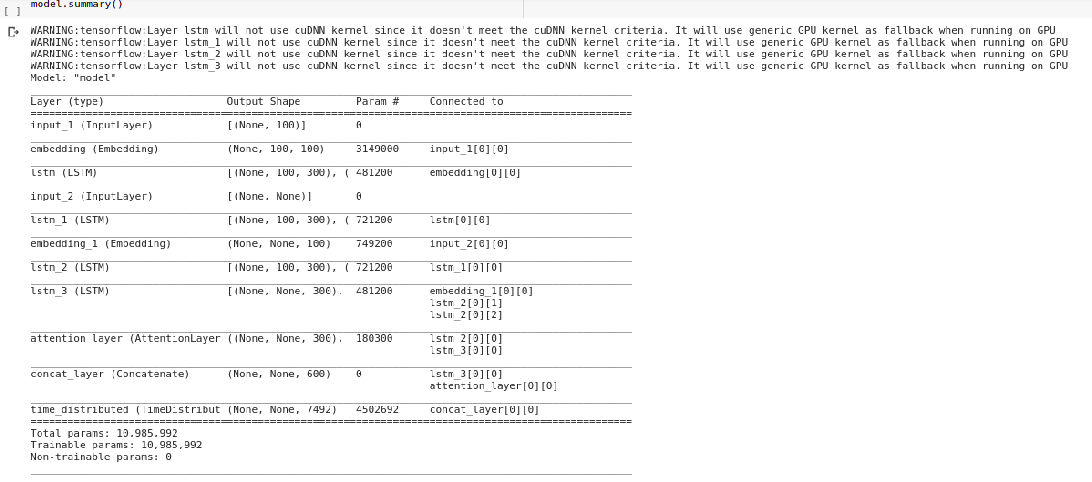
\includegraphics[scale=0.45]{images/model_training1.png}
\caption{Seq2Seq Model with Attention Mechanism Architecture}
\label{fig:train}
\end{figure}

\begin{figure}[H]
\centering
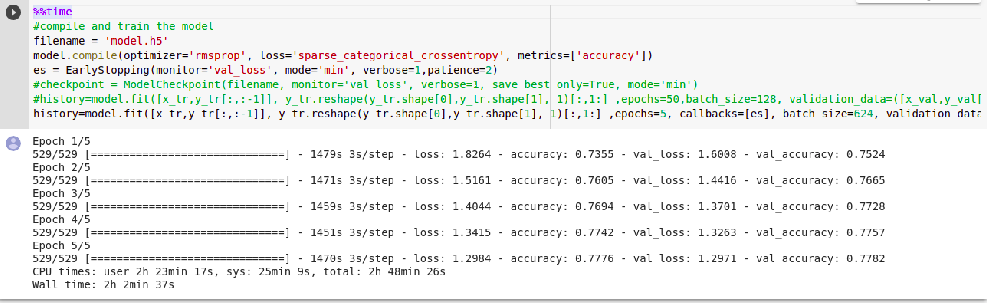
\includegraphics[scale=0.5]{images/model_training0.png}
\caption{Model Training}
\label{fig:train}
\end{figure}

\begin{figure}[H]
\centering
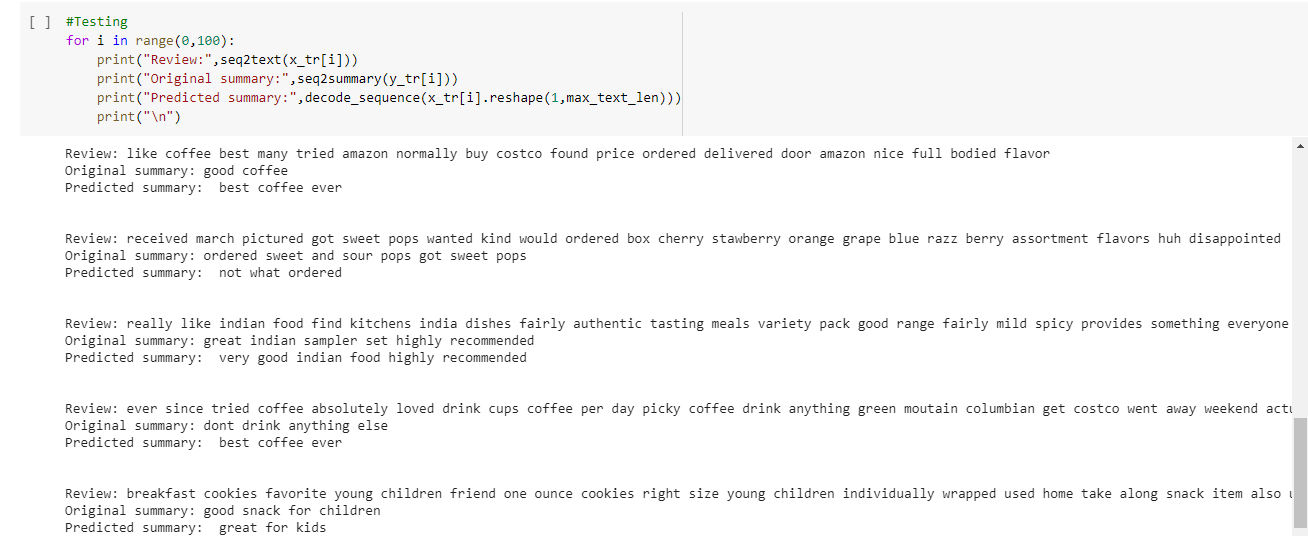
\includegraphics[scale=0.5]{images/predicted summary.png}
\caption{Summaries Predicted by Trained Model}
\label{fig:train}
\end{figure}

\newpage
\subsection{Summary Generation \& Sentiment Analysis}
Preprocessed data is fed into the trained seq2seq model and trained naive bayes model. The models generate an abstractive summary and the predict the sentiment respectively, which is then given to the web application. The web application displays the generated summary along with the sentiment and review rating for the user to view.
\begin{figure}[H]
\centering
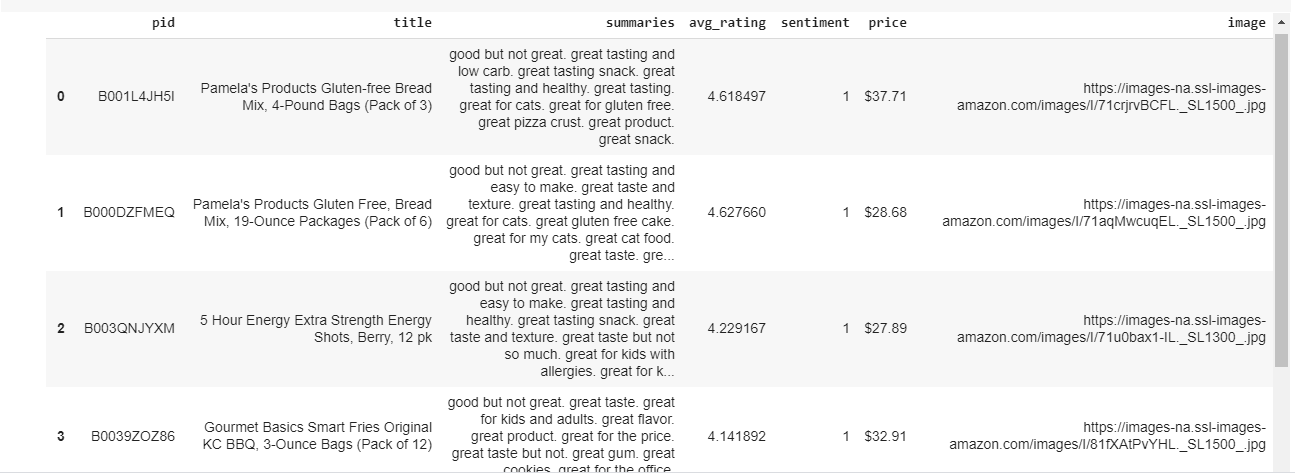
\includegraphics[scale=0.5]{images/SummaryGeneration.png}
\caption{Final Summary, Sentiment and Average Rating}
\label{fig:summaryfinal}
\end{figure}

\section{Integration Testing}
Integration testing refers to the testing of the different modules/components that have been successfully unit tested when integrated together to perform specific tasks and activities. The purpose of integration testing is to detect any inconsistencies between the units that are integrated together.
\begin{figure}[H]
\centering
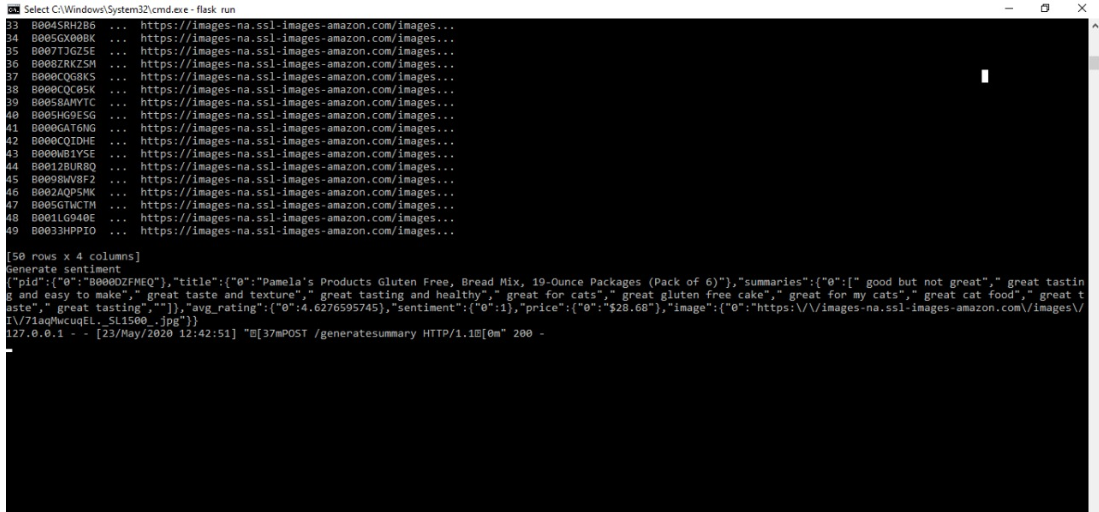
\includegraphics[scale=0.5]{images/IntegrationTesting.png}
\caption{Generated Summary}
\label{fig:integration}
\end{figure}

\section{System Testing}
The system testing part of a testing methodology involves testing the complete system for errors and bugs. All modules were integrated at the end of integration testing and the entire system is tested here.
\begin{figure}[H]
\centering
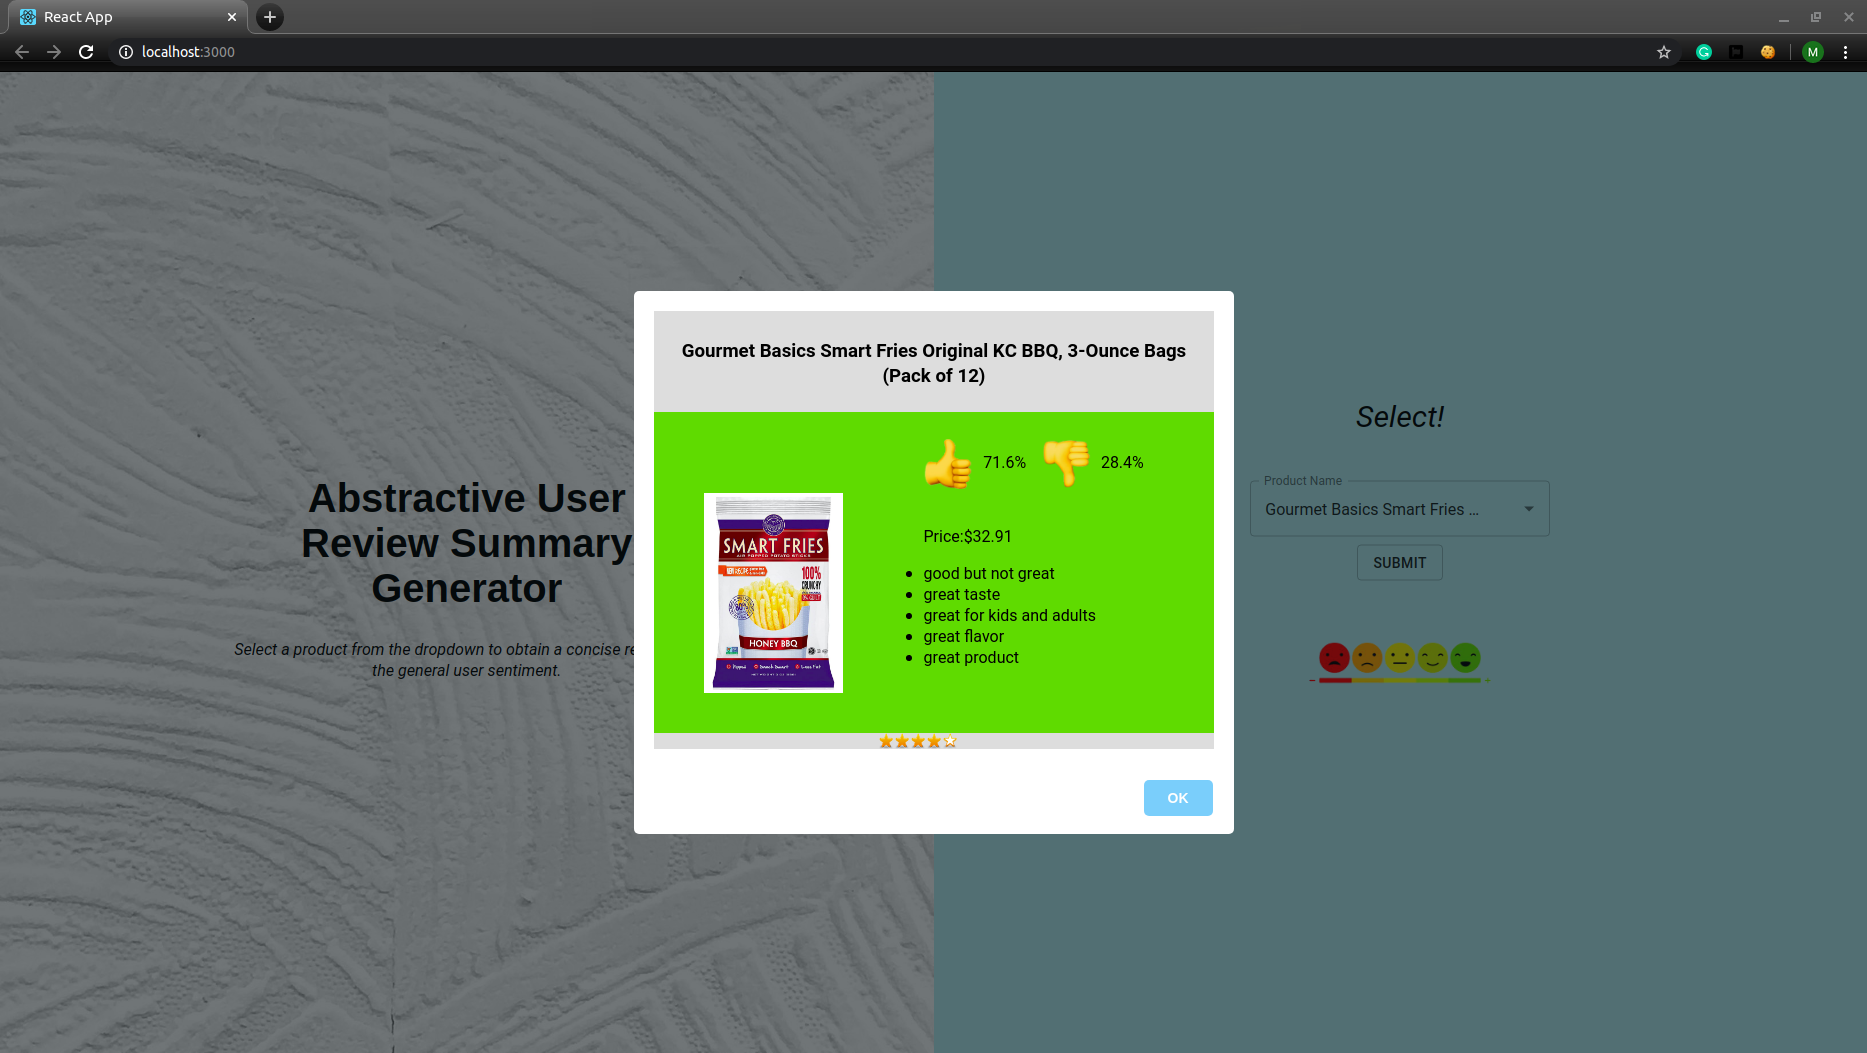
\includegraphics[scale=0.27]{images/FinalOutput.png}
\caption{Abstractive Summarization System}
\label{fig:finaloutput}
\end{figure}


\newpage
\section{Validation Testing}
The system is compared to Text Compactor (https://www.textcompactor.com/) which is a free online automatic text summarization tool. The tool has an input box to enter the text. It provides an option to specify the percentage of the text to be retained within the summary. 
\begin{figure}[H]
    \centering
    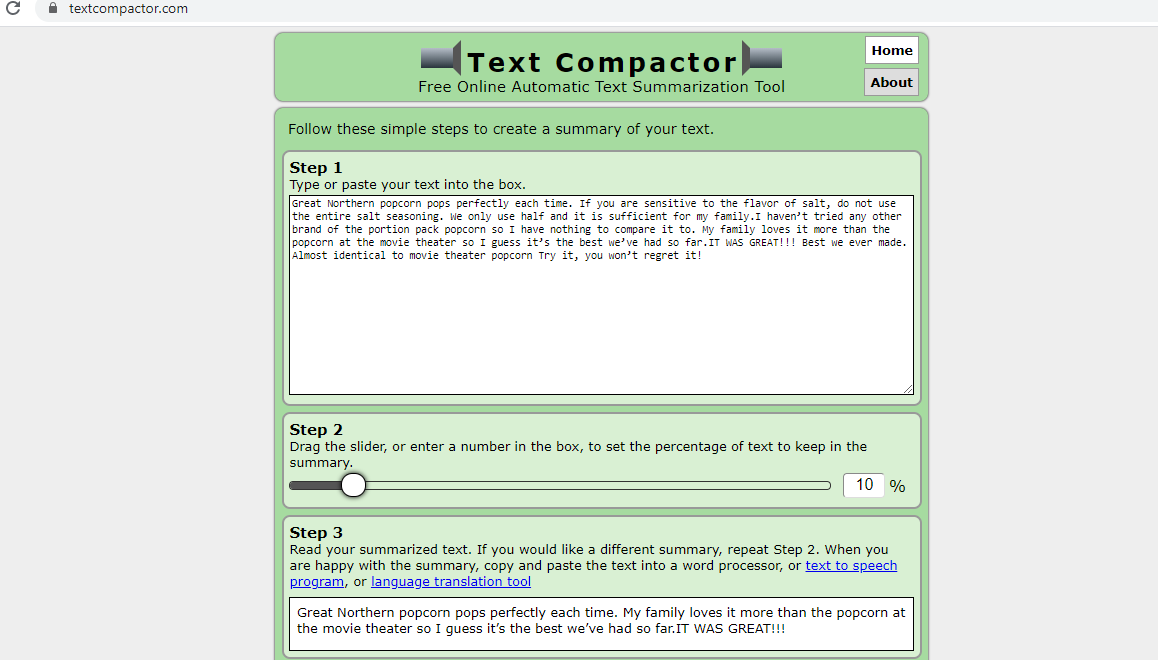
\includegraphics[scale=0.5]{images/ValidationTesting.png}
    \caption{Summarization using Text Compactor}
    \label{fig:my_label}
\end{figure}


In comparison to the Text Compactor which uses extractive summarization, the developed system uses abstractive summarization, thereby producing new sentences. These sentences contain the gist of the whole of the content, represented as points, in contrast to limiting the content by a percentage.The software used for testing only provides selected sentences from the input text based on the frequency of the repeated words, without knowing the relevance of the same in the given text.

The developed system understands the context of the text and prepares a sentence on its own. It also provides the overall sentiment of the reviews, as a percentage of positive and negative review along with the overall rating.

\chapter{Graphical User Interface}
\section{GUI Overview}
The user interface is quite simple and straight-forward. The home page gives you the option to select the product from an auto-complete drop-down list. On selecting the product, a sweet alert appears with the summary of the reviews, image, sentiment and rating of the product that was selected.
\section{Main GUI Components}
\begin{figure}[H]
\centering
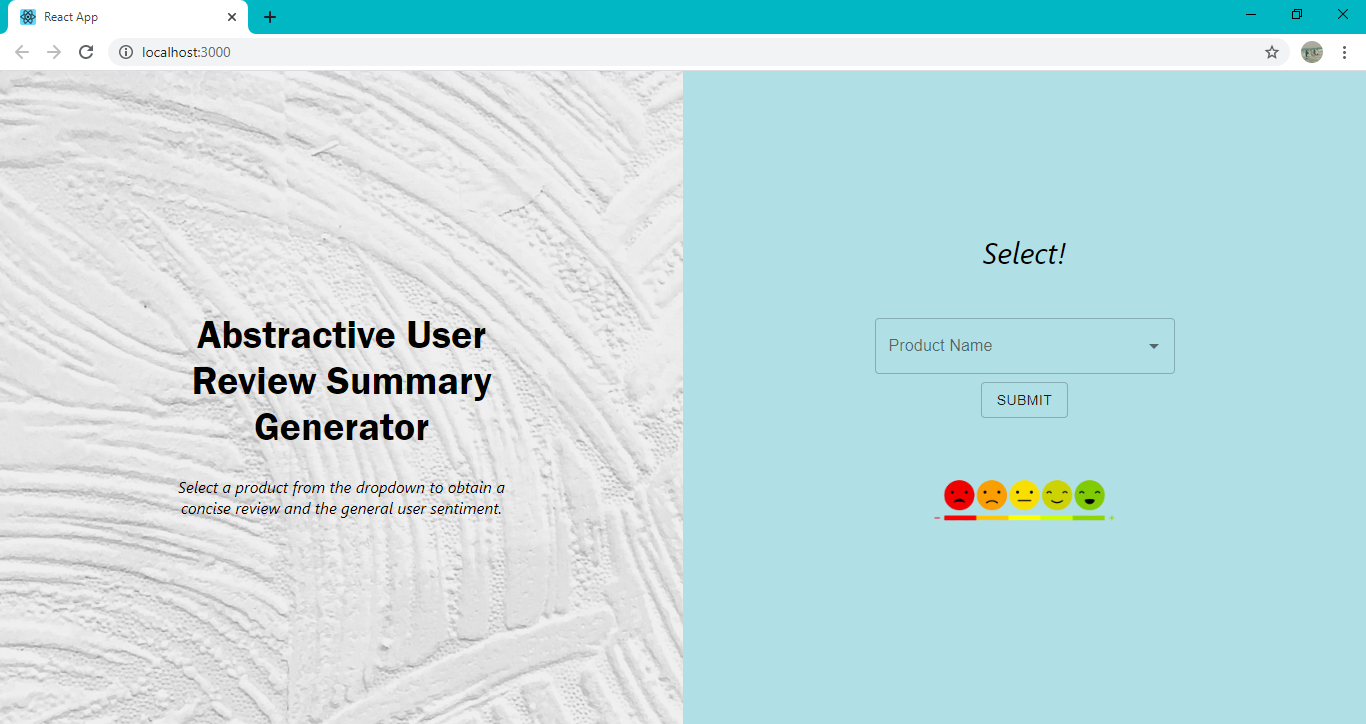
\includegraphics[scale=0.45]{images/homepage.png}
\caption{GUI Interface}
\label{fig:homepage}
\end{figure}
The user interface gives you the options to select the product from the auto complete drop-down list.\\

\begin{figure}[H]
\centering
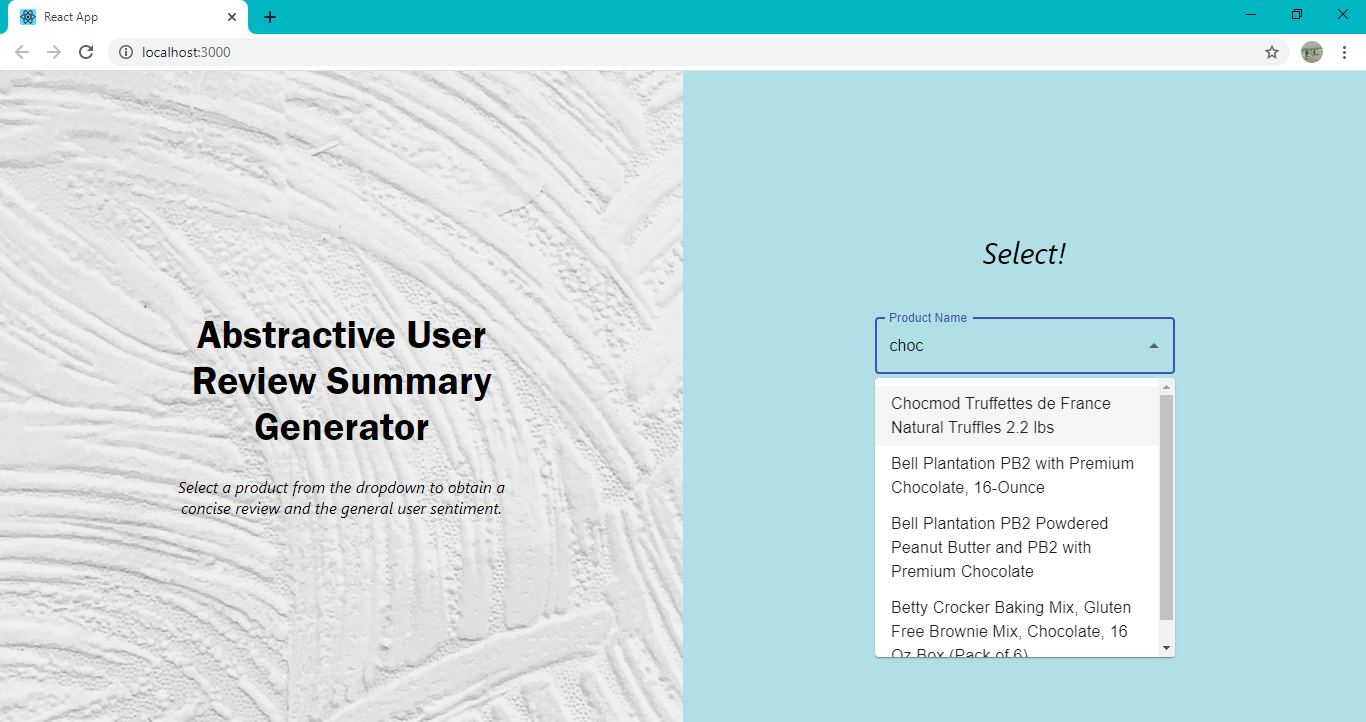
\includegraphics[scale=0.42]{images/dropdown.png}
\caption{Drop-Down Selection}
\label{fig:dropdown}
\end{figure}
After selecting the product, the summary is generated along with the rating, sentiment and the image of the product in a sweet alert. 

\begin{figure}[hbt!]
\centering
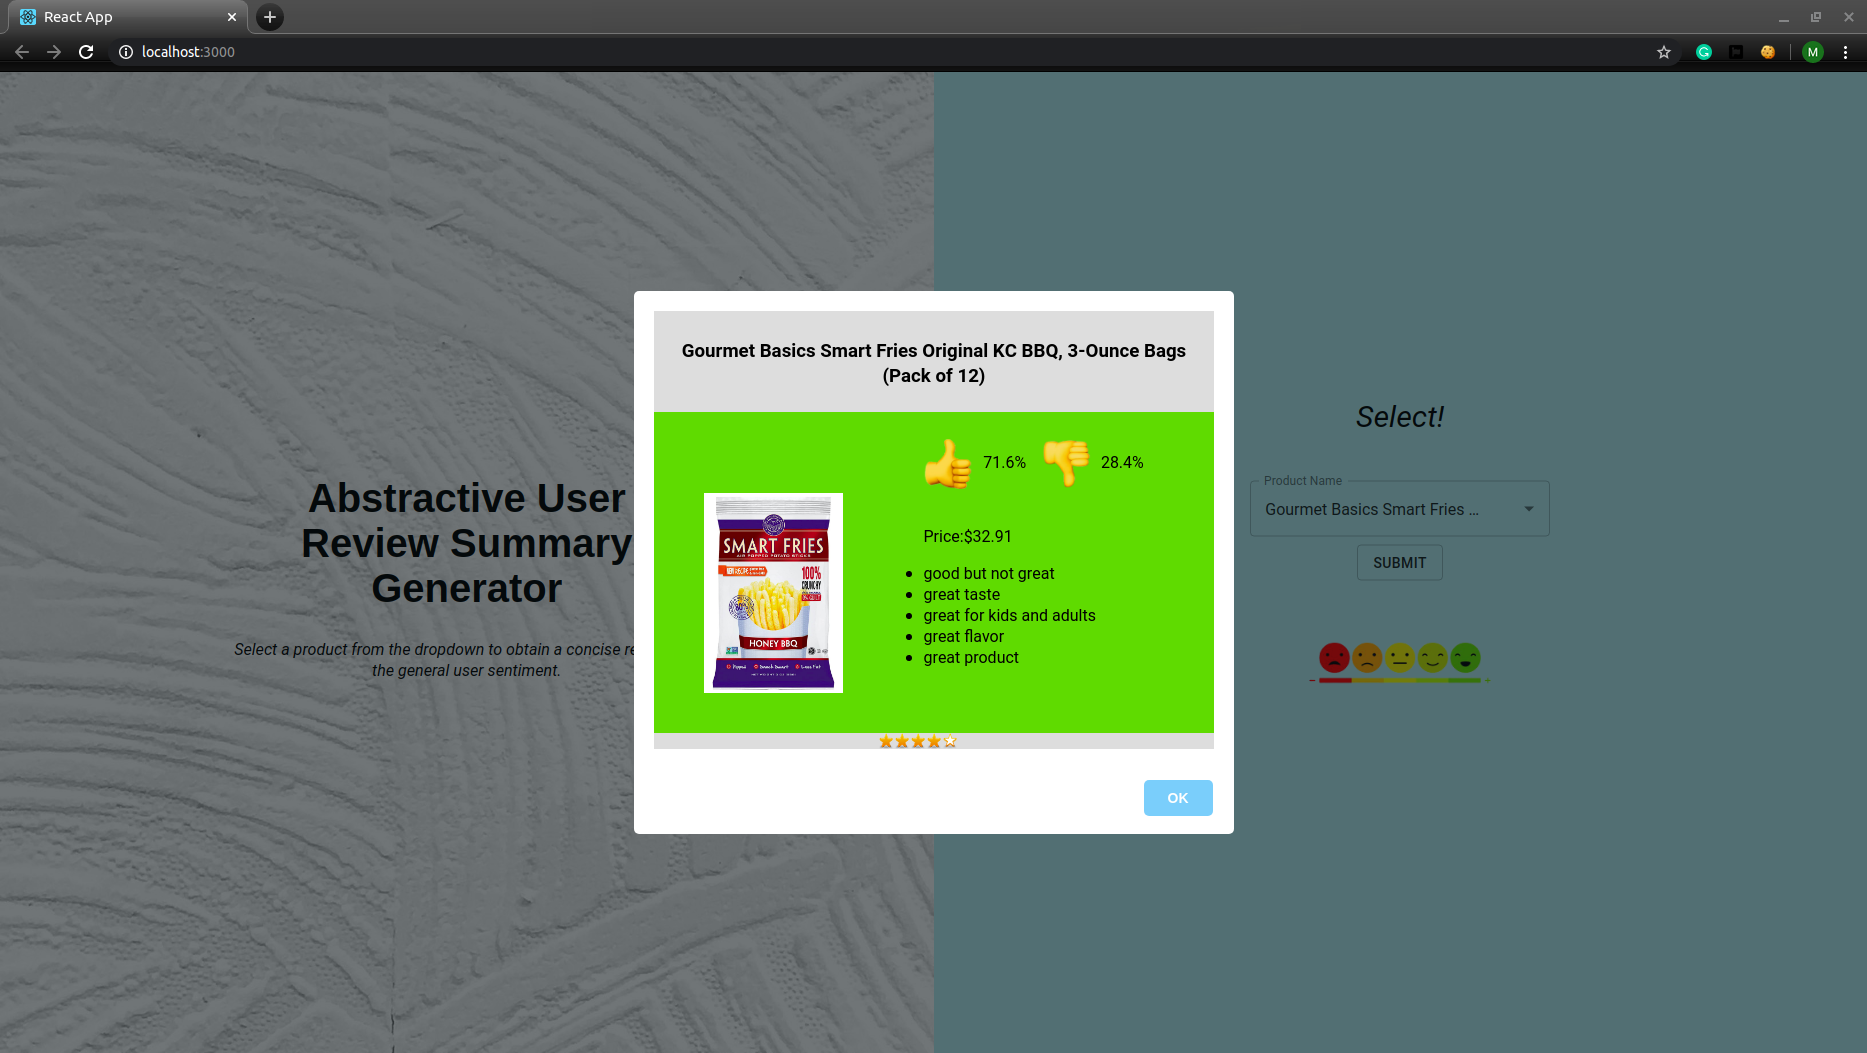
\includegraphics[scale=0.23]{images/FinalOutput.png}
\caption{SweetAlert}
\label{fig:output}
\end{figure}

\chapter{Results}
The web application for the system displays an auto-complete drop-down list in which users can type in the product name. On hitting the submit button, the product id of the selected product is passed onto the back-end of the application. 
\begin{figure}[H]
\centering
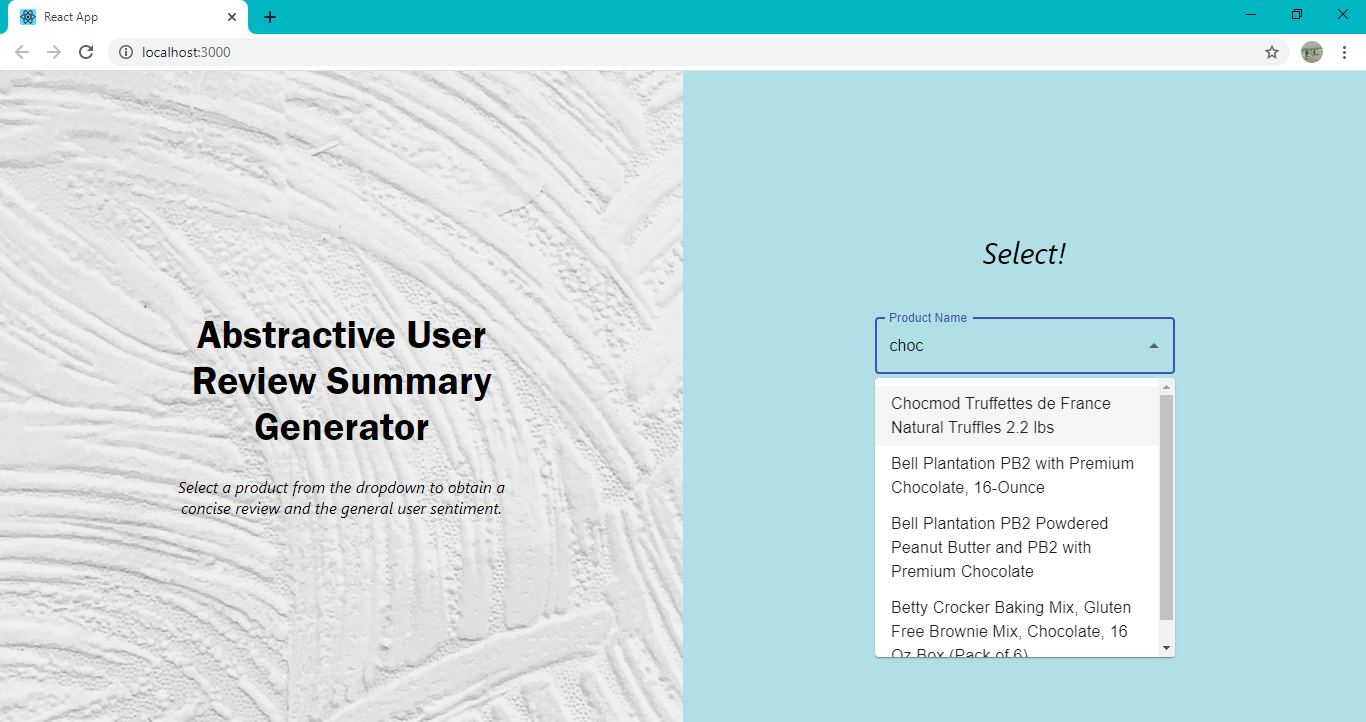
\includegraphics[scale=0.5]{images/dropdown.png}
\caption{Input Selection}
\label{fig:input}
\end{figure}

At the back-end, the reviews of the product are selected and preprocessed. This is then to the trained Naive Bayes model to generate the sentiment of each review. The percentage of positive and negative reviews is calculated. The reviews are also passed into the trained deep learning model for summary generation. The summaries, along with the sentiment percentage and the average rating is returned to the front-end to be viewed by the user.
\begin{figure}[hbt!]
\centering
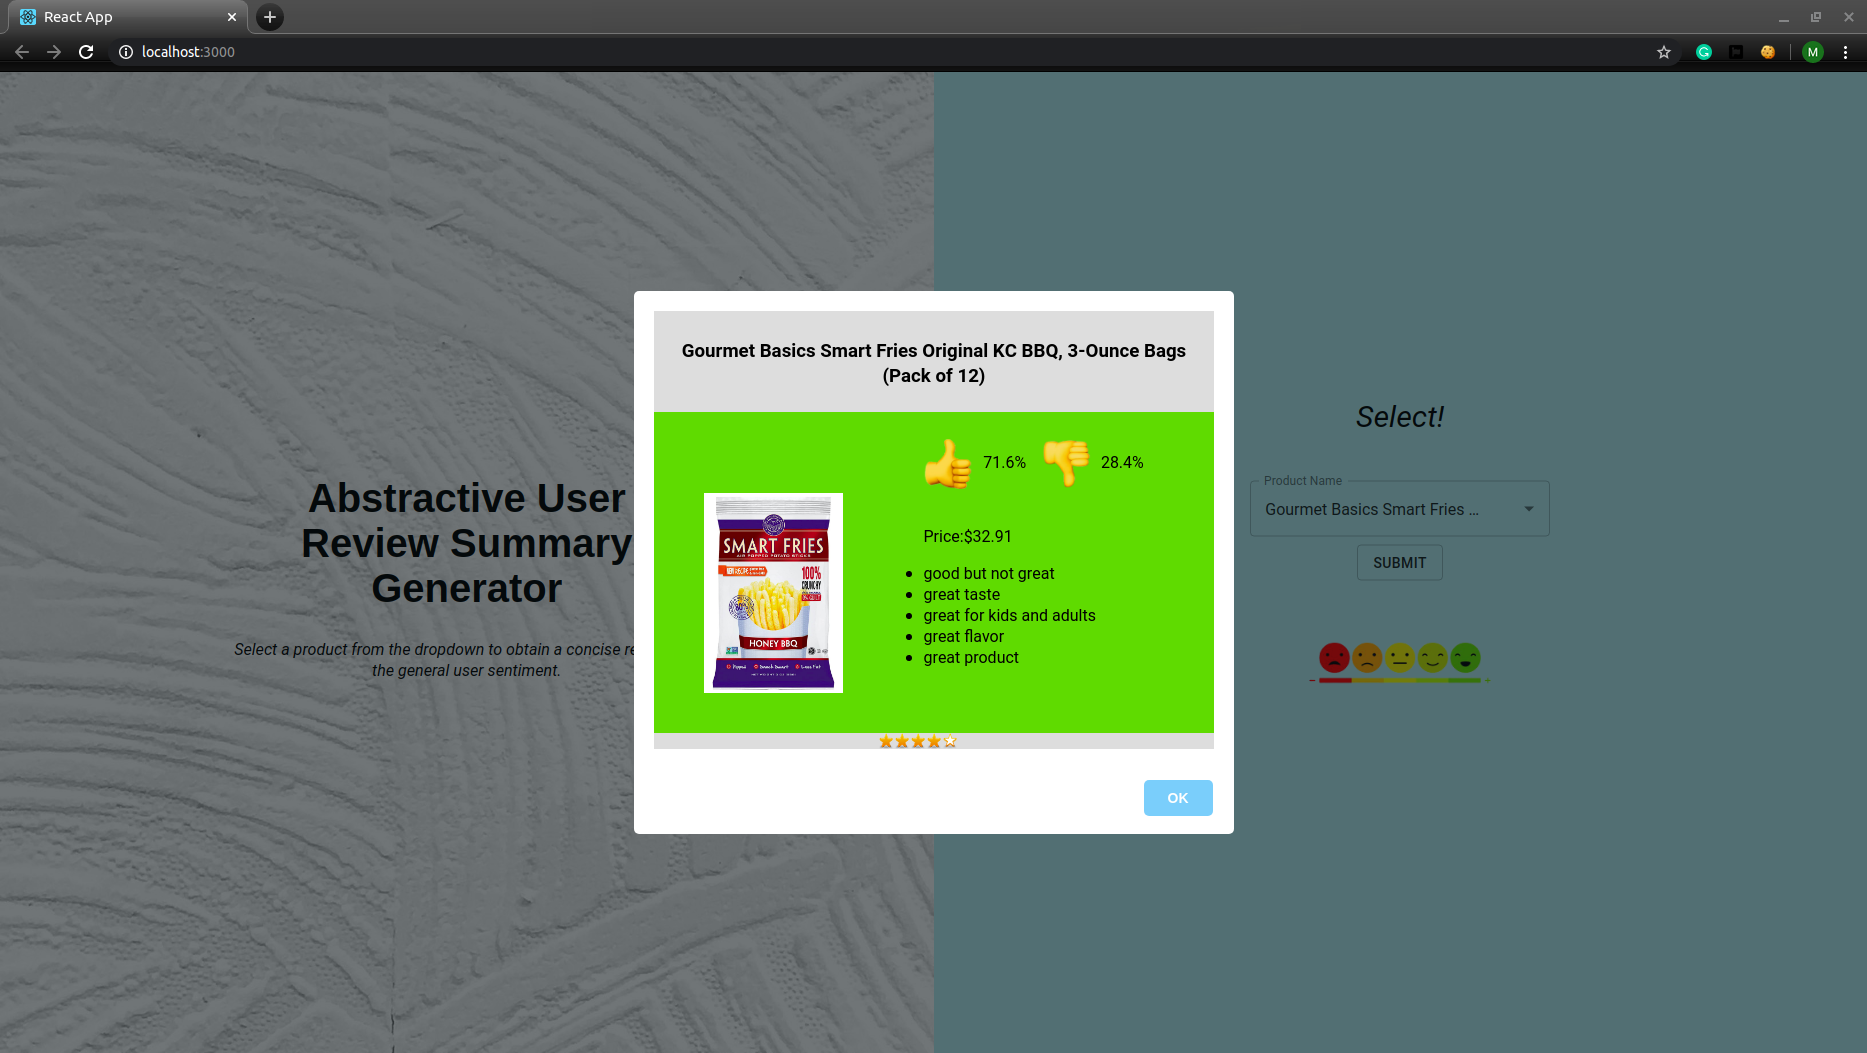
\includegraphics[scale=0.27]{images/FinalOutput.png}
\caption{Generated Abstractive Summary}
\label{fig:output}
\end{figure}
\newpage
The response from the back-end application which includes the summaries, sentiment percentage and the average rating is displayed using a sweet alert box. The alert box features the product name, image and price and the summaries as a bulleted list. The thumbs-up and thumbs-down images indicate the percentage of positive and negative reviews respectively. The filled stars on the bottom represent the average rating out of 5 and the background colour also depicts the range of the product rating. 

\chapter{Conclusion}
A user review consolidation system has been developed using the method of abstractive summarizing to obtain a concise form of the lengthy product reviews available on e-commerce websites along with additional features such as overall rating and sentiment analysis. The system uses a dataset of fine food reviews from E-commerce websites to generate the summaries. It also generates the general sentiment of the customers towards each product. The average rating based on the numerous reviews available for each product is also calculated.\\ \\
The sentiment analysis has been performed by training a model based on supervised learning. The Naive Bayes classifier has been chosen as the machine learning model, trained on social-media sentiment analysis data, which provides an accuracy of more than 95\%. The abstractive summarizer has been modelled as a Sequence-to-Sequence model which uses attention mechanism to improve accuracy. The model gives fairly good summaries of the reviews. 

\chapter{Future Scope}
The model is trained using reviews for a selected dataset. It can be extended to include other categories of items available online, thereby generating better summaries due to a larger dataset. It can also be improved to integrate reviews from various other online shopping websites to provide an unbiased summary and rating.\\ \\
The generalization capability of a deep learning model enhances with an increase in the training dataset size. Web scraping can be introduced to perform summarization on real-time data.\\ \\
Implementing Bi-Directional LSTM which is capable of capturing the context from both the directions could result in a better context vector. The beam search strategy can be applied for decoding the test sequence instead of using the greedy approach (argmax). Pointer-generator networks and coverage mechanisms can be implemented in the model to further improve the summary generation capability of the model.

%\chapter{Publication}
   
\begin{thebibliography}{999}
\addcontentsline{toc}{chapter}{References}


\bibitem[1]{1}Chetana Badgujar, Vimla Jethani and Tushar Ghorpade ”Abstractive Summarization using Graph Based Methods” Proceedings of the 2nd International Conference on Inventive Communication and Computational Technologies (ICICCT 2018), IEEE 2018

\bibitem[2]{2}Moye Chen, Lei Li, Wei Liu ”A Multi-View Abstractive Summarization Model Jointly Considering Semantics and Sentiment”, Proceedings of CCIS2018

\bibitem[3]{3}Tooba Siddiqui, Jawwad Ahmed Shamsi ”Generating Abstractive Summaries Using Sequence to Sequence Attention Model”, 2018 International Conference on Frontiers of Information Technology (FIT)

\bibitem[4]{4}Ranjitha N S, Dr. Jagadish S Kallimani ”Abstractive Multi-Document Summarization”

\bibitem[5]{5}A.Jeyapriya, C.S.Kanimozhi Selvi ”Extracting Aspects and Mining Opinions inProduct Reviews using Supervised Learning Algorithm”, IEEE Sponsored 2nd International Conference On Electronics And Communication Systems(ICECS 2015)

\bibitem[6]{6}Wenbo Nie, Wei Zhang, Xinle Li, Yao Yu ”An Abstractive Summarizer Based on Improved Pointer-Generator Network”

\bibitem[7]{7}Kaichun Yao, Libo Zhang , Dawei Du , Tiejian Luo, Lili Tao, and Yanjun Wu ”Dual Encoding for Abstractive Text Summarization”, IEEE Transactions on Cybernetics

\bibitem[8]{8}Alshaina S, Ansamma John, Aneesh G Nath ”Multi-document Abstractive Summarization Based on Predicate Argument Structure”

\bibitem[9]{9}Farshad Kiyoumarsi ”Evaluation Of Automatic Text Summarizations Based On Human Summaries”, 2nd Global Conference on Linguistics and Foreign Language Teaching LINELT-2014

\bibitem[10]{10}Atif Khan, Naomie Salim, Haleem Farman ”Clustered Genetic Semantic Graph Approach for Multi-document Abstractive Summarization”

\bibitem[11]{11}Shuai Wang, Xiang Zhao, Bo Li, Bin Ge, Daquan Tang ”Integrating Extractive and Abstractive Models for Long Text Summarization”, 2017 IEEE 6th International Congress on Big Data

\bibitem[12]{12}Siddhartha Banerjee, Prasenjit Mitra, Kazunari Sugiyama ”Multi Document Abstractive summarization using ILP Based Multi Sentence Compression”

\bibitem[13]{13} Alexander M. Rush, Sumit Chopra, Jason Weston ”A Neural Attention Model for Abstractive Sentence Summarization”, Proceedings of the 24th International Joint Conference on Artificial Intelligence (IJCAI-2015)

\bibitem[14]{14}Jianwei Niu, Huan Chen, Qingjuan Zhao, Limin Sun†, Mohammed Atiquzzaman ”Multi-Document Abstractive Summarization using Chunk-graph and Recurrent Neural Network”, IEEE ICC 2017 SAC Symposium Big Data Networking Track

\bibitem[15]{15}Hao Xu, Yanan Cao, Ruipeng Jia, Yanbing Liu, Jianlong Tan ”Sequence Generative Adversarial Network for Long Text Summarization”, 2018 IEEE 30th International Conference on Tools with Artificial Intelligence

\bibitem[16]{16}Harsha Dave, Shree Jaswal ”Multiple Text Document Summarization System using Hybrid Summarization Technique”, 2015 1st International Conference on Next Generation Computing Technologies

\bibitem[17]{17}Jagbir Kaur, Meenakshi Bansal ”Multi-Layered Sentiment Analytical Model for Product Review Mining”, 2016 Fourth International Conference on Parallel, Distributed and Grid Computing

\bibitem[18]{18}Allahyari, Mehdi, et al. “Text Summarization Techniques: A Brief Survey.” arXiv preprint arXiv:1707.02268 2017.

\bibitem[19]{19}Yao, Jin-ge, Xiaojun Wan, and Jianguo Xiao. “Recent advances in document summarization” Knowledge and Information Systems: 140 2017.

\bibitem[20]{20}https://www.kaggle.com/snap/amazon-fine-food-reviews/home

\bibitem[21]{21}Khan, Atif, and Naomie Salim. “A review on abstractive summarization methods.”Journal of Theoretical and Applied Information Technology 59.1: 64-72, 2014

\bibitem[22]{22}Dalal, Vipul, and Latesh G. Malik. “A survey of extractive and abstractive text summarization techniques.” 2013 6th International Conference on Emerging Trends in Engineering and Technology (ICETET), . IEEE, 2013.

\bibitem[23]{23}Vilca, Gregory Csar Valderrama, and Marco Antonio Sobrevilla Cabezudo. “A Study of Abstractive Summarization Using Semantic Representations and Discourse Level Information.” International Conference on Text, Speech, and Dialogue. Springer, Cham 2017.

\bibitem[24]{24}Moratanch, N., and S. Chitrakala. “A survey on abstractive text summarization” Circuit, International Conference on Power and Computing Technologies(ICCPCT), IEEE 2016.

\bibitem[25]{25}Shimpikar, Sheetal, and Sharvari Govilkar “A Survey of Text Summarization Techniques for Indian Regional Languages” International Journal of Computer Applications 165.112017

\bibitem[26]{26}Ganesan, Kavita, ChengXiang Zhai, and Jiawei Han. “Opinosis: a graph based approach to abstractive summarization of highly redundant opinions” Proceedings of the 23rd international conference on computational linguistics. Association for
Computational Linguistics 2010

\bibitem[27]{27}Lloret, Elena and Manuel Palomar. “Analyzing the use of word graphs for abstractive text summarization” Proceedings of the First International Conference on Advances in Information Mining and Management, Barcelona, Spain 2011.

\bibitem[28]{28}Kumar, Niraj, Kannan Srinathan and Vasudeva Varma. “A knowledge induced graph-theoretical model for extract and abstract single document summarization” International Conference on Intelligent Text Processing and Computational Linguistics. Springer, Berlin, Heidelberg 2013.

\bibitem[29]{29}Subramaniam, Manjula and Vipul Dalal.“Test Model for Rich Semantic Graph Representation for Hindi Text using Abstractive Method” 2015.

\bibitem[30]{30}Liu, Fei, et al. “Toward abstractive summarization using semantic representa-tions.”1077,2015

\bibitem[31]{31}Bhargava, Rupal, Yashvardhan Sharma, and Gargi Sharma. “ATSSI: Abstractive Text Summarization Using Sentiment Infusion.” Procedia Computer Science 89,404-411 2016

\bibitem[32]{32}Eduard Hovy, Mitchell Marcus, Martha Palmer, Lance Ramshaw, and Ralpheischedel. OntoNotes: The 90 solution. In Proceedings of NAACL,2006
 
\bibitem[33]{33}Sunitha C, Dr. A Jaya and Amal Ganesh “Abstractive Summarization Techniques in Indian Languages” Peer-review under responsibility of the Organizing Committee of ICRTCSE 2016 doi: 10.1016/j.procs.2016.05.121, International Conference of recent trends in computer science., 2016

\end{thebibliography}

\end{document}
